%%%%%%%%%%%%%%%%%%%%%%%%%%%%%%%%%%%%%%%%%%%%%%%%%%%%%%%%%%%%%%%%%%%%%%%%%%%%%%%%
%%%%%%%%%%%%%%%%%%%%%%%%%%%%%%%%%%%%%%%%%%%%%%%%%%%%%%%%%%%%%%%%%%%%%%%%%%%%%%%%
%%                                                                            %%
%% thesistemplate.tex version 3.10 (2018/04/24)                               %%
%% The LaTeX template file to be used with the aaltothesis.sty (version 3.10) %%
%% style file.                                                                %%
%% This package requires pdfx.sty v. 1.5.84 (2017/05/18) or newer.            %%
%%                                                                            %%
%% This is licensed under the terms of the MIT license below.                 %%
%%                                                                            %%
%% Copyright 2017-2018, by Luis R.J. Costa, luis.costa@aalto.fi,              %%
%% Copyright 2017-2018 documentation in Finnish in the template by Perttu     %%
%% Puska, perttu.puska@aalto.fi                                               %%
%% Copyright Swedish translations 2017-2018 by Elisabeth Nyberg,              %%
%% elisabeth.nyberg@aalto.fi and Henrik Wallén, henrik.wallen@aalto.fi        %%
%%                                                                            %%
%% Permission is hereby granted, free of charge, to any person obtaining a    %%
%% copy of this software and associated documentation files (the "Software"), %%
%% to deal in the Software without restriction, including without limitation  %%
%% the rights to use, copy, modify, merge, publish, distribute, sublicense,   %%
%% and/or sell copies of the Software, and to permit persons to whom the      %%
%% Software is furnished to do so, subject to the following conditions:       %%
%% The above copyright notice and this permission notice shall be included in %%
%% all copies or substantial portions of the Software.  \textbf{•}                      %%
%% THE SOFTWARE IS PROVIDED "AS IS", WITHOUT WARRANTY OF ANY KIND, EXPRESS OR %%
%% IMPLIED, INCLUDING BUT NOT LIMITED TO THE WARRANTIES OF MERCHANTABILITY,   %%
%% FITNESS FOR A PARTICULAR PURPOSE AND NONINFRINGEMENT. IN NO EVENT SHALL    %%
%% THE AUTHORS OR COPYRIGHT HOLDERS BE LIABLE FOR ANY CLAIM, DAMAGES OR OTHER %%
%% LIABILITY, WHETHER IN AN ACTION OF CONTRACT, TORT OR OTHERWISE, ARISING    %%
%% FROM, OUT OF OR IN CONNECTION WITH THE SOFTWARE OR THE USE OR OTHER        %%
%% DEALINGS IN THE SOFTWARE.                                                  %%
%%                                                                            %%
%%                                                                            %%
%%%%%%%%%%%%%%%%%%%%%%%%%%%%%%%%%%%%%%%%%%%%%%%%%%%%%%%%%%%%%%%%%%%%%%%%%%%%%%%%
%%                                                                            %%
%%                                                                            %%
%% An example for writting your thesis using LaTeX                            %%
%% Original version and development work by Luis Costa, changes by Perttu     %% 
%% Puska.                                                                     %%
%% Support for Swedish added 15092014                                         %%
%% PDF/A-b support added on 15092017                                          %%
%% PDF/A-2b and PDF/A-3b support added on 24042018                            %%
%%                                                                            %%
%% This example consists of the files                                         %%
%%         thesistemplate.tex (versio 3.10)                                   %%
%%         opinnaytepohja.tex (versio 3.10) (for text in Finnish)             %%
%%         aaltothesis.cls (versio 3.10)                                      %%
%%         kuva1.eps (graphics file)                                          %%
%%         kuva2.eps (graphics file)                                          %%
%%         kuva1.jpg (graphics file)                                          %%
%%         kuva2.jpg (graphics file)                                          %%
%%         kuva1.png (graphics file)                                          %%
%%         kuva2.png (graphics file)                                          %%
%%         kuva1.pdf (graphics file)                                          %%
%%         kuva2.pdf (graphics file)                                          %%
%%                                                                            %%
%%                                                                            %%
%% Typeset in Linux either with                                               %%
%% pdflatex: (recommended method)                                             %%
%%             $ pdflatex thesistemplate                                      %%
%%             $ pdflatex thesistemplate                                      %%
%%                                                                            %%
%%   The result is the file thesistemplate.pdf that is PDF/A compliant, if    %%
%%   you have chosen the proper \documenclass options (see comments below)    %%
%%   and your included graphics files have no problems.
%%                                                                            %%
%% Or                                                                         %%
%% latex:                                                                     %%
%%             $ latex thesistemplate                                         %%
%%             $ latex thesistemplate                                         %%
%%                                                                            %%
%%   The result is the file thesistemplate.dvi, which is converted to ps      %%
%%   format as follows:                                                       %%
%%                                                                            %%
%%             $ dvips thesistemplate -o                                      %%
%%                                                                            %%
%%   and then to pdf as follows:                                              %%
%%                                                                            %%
%%             $ ps2pdf thesistemplate.ps                                     %%
%%                                                                            %%
%%   This pdf file is not PDF/A compliant. You must must make it so using,    %%
%%   e.g., Acrobat Pro or PDF-XChange.                                        %%
%%                                                                            %%
%%                                                                            %%
%% Explanatory comments in this example begin with the characters %%, and     %%
%% changes that the user can make with the character %                        %%
%%                                                                            %%
%%%%%%%%%%%%%%%%%%%%%%%%%%%%%%%%%%%%%%%%%%%%%%%%%%%%%%%%%%%%%%%%%%%%%%%%%%%%%%%%
%%%%%%%%%%%%%%%%%%%%%%%%%%%%%%%%%%%%%%%%%%%%%%%%%%%%%%%%%%%%%%%%%%%%%%%%%%%%%%%%
%%
%% WHAT is PDF/A
%%
%% PDF/A is the ISO-standardized version of the pdf. The standard's goal is to
%% ensure that he file is reproducable even after a long time. PDF/A differs
%% from pdf in that it allows only those pdf features that support long-term
%% archiving of a file. For example, PDF/A requires that all used fonts are
%% embedded in the file, whereas a normal pdf can contain only a link to the
%% fonts in the system of the reader of the file. PDF/A also requires, among
%% other things, data on colour definition and the encryption used.
%% Currently three PDF/A standards exist:
%% PDF/A-1: based on PDF 1.4, standard ISO19005-1, published in 2005.
%%          Includes all the requirements essential for long-term archiving.
%% PDF/A-2: based on PDF 1.7, standard ISO19005-2, published in 2011.
%%          In addition to the above, it supports embedding of OpenType fonts,
%%          transparency in the colour definition and digital signatures.
%% PDF/A-3: based on PDF 1.7, standard ISO19005-3, published in 2012.
%%          Differs from the above only in that it allows embedding of files in
%%          any format (e.g., xml, csv, cad, spreadsheet or wordprocessing
%%          formats) into the pdf file.
%% PDF/A-1 files are not necessarily PDF/A-2 -compatible and PDF/A-2 are not
%% necessarily PDF/A-1 -compatible.
%% All of the above PDF/A standards have two levels:
%% b: (basic) requires that the visual appearance of the document is reliably
%%    reproduceable.
%% a (accessible) in addition to the b-level requirements, specifies how
%%   accessible the pdf file is to assistive software, say, for the physically
%%   impaired.
%% For more details on PDF/A, see, e.g., https://en.wikipedia.org/wiki/PDF/A
%%
%%
%% WHICH PDF/A standard should my thesis conform to?
%%
%% Primarily to the PDF/A-1b standard. All the figures and graphs typically
%% use in thesis work do not require transparency features, a basic '2-D'
%% visualisation suffices. The font to be used are specified in this template
%% and they should not be changed. However, if you have figures where
%% transparency characteristics matter, use the PDF/A-2b standard. Do not use
%% the PDF/A-3b standard for your thesis.
%%
%%
%% WHAT graphics format can I use to produce my PDF/A compliant file?
%%
%% When using pdflatex to compile your work, use jpg, png or pdf files. You may
%% have PDF/A compliance problems with figures in pdf format. Do not use PDF/A
%% compliant graphics files.
%% If you decide to use latex to compile your work, the only acceptable file
%% format for your figure is eps. DO NOT use the ps format for your figures.

%% USE one of these:
%% * the first when using pdflatex, which directly typesets your document in the
%%   chosen pdf/a format and you want to publish your thesis online,

%% * the second when you want to print your thesis to bind it, or
%% * the third when producing a ps file and a pdf/a from it.
%%
\documentclass[english, 12pt, a4paper, elec, utf8, online]{aaltothesis}
%\documentclass[english, 12pt, a4paper, elec, utf8, a-1b]{aaltothesis}
%\documentclass[english, 12pt, a4paper, elec, dvips, online]{aaltothesis}

%% Use the following options in the \documentclass macro above:
%% your school: arts, biz, chem, elec, eng, sci
%% the character encoding scheme used by your editor: utf8, latin1
%% thesis language: english, finnish, swedish
%% make an archiveable PDF/A-1b, PDF/A-2b or PDF/A-3b compliant file: a-1b,
%%                    a-2b, a-3b
%%                    (a normal pdf is produced without the a-*b option)
%% typeset in symmetric layout and blue hypertext for online publication: online
%%            (no option is the default, resulting in a wide margin on the
%%             binding side of the page and black hypertext)
%% two-sided printing: twoside (default is one-sided printing)
%%

%% Use one of these if you write in Finnish (see the Finnish template
%% opinnaytepohja.tex)
%\documentclass[finnish, 12pt, a4paper, elec, utf8, a-1b, online]{aaltothesis}
%\documentclass[finnish, 12pt, a4paper, elec, utf8, a-1b]{aaltothesis}
%\documentclass[finnish, 12pt, a4paper, elec, dvips, online]{aaltothesis}



%% Math fonts, symbols, and formatting; these are usually needed
\usepackage{amsfonts,amssymb,amsbsy}
\usepackage{amsmath}
\usepackage{multirow}
\usepackage{longtable}
\usepackage{graphicx}
\usepackage{tikz} 
\usetikzlibrary{shapes,arrows,spy,positioning,snakes}
\usetikzlibrary{calc}
\usepackage{caption}
\usepackage{subcaption}
\usepackage{listings}
\usepackage{protobuf/lang}  % include language definition for protobuf
\usepackage{protobuf/style} % include custom style for proto declarations.

\usepackage{pgfplots}
\usetikzlibrary{datavisualization}

\usepackage{physics}

\usepackage{color}
\definecolor{gray}{rgb}{0.4,0.4,0.4}
\definecolor{darkblue}{rgb}{0.0,0.0,0.6}
\definecolor{cyan}{rgb}{0.0,0.6,0.6}

\lstset{
  basicstyle=\ttfamily,
  columns=fullflexible,
  showstringspaces=false,
  commentstyle=\color{gray}\upshape
}

\lstdefinelanguage{XML}
{
  morestring=[b]",
  morestring=[s]{>}{<},
  morecomment=[s]{<?}{?>},
  stringstyle=\color{black},
  identifierstyle=\color{darkblue},
  keywordstyle=\color{cyan},
  morekeywords={xmlns,version,type}% list your attributes here
}


\DeclareMathOperator*{\argmax}{argmax} % thin space, limits underneath in displays
\DeclareMathOperator*{\argmin}{argmin}
%% Change the school field to specify your school if the automatically set name
%% is wrong
% \university{aalto-yliopisto}
% \school{Sähkötekniikan korkeakoulu}

%% Edit to conform to your degree programme
%%
\degreeprogram{Master's Programme in Automation and Electrical Engineering}
%%

%% Your major
%%
\major{Control, Robotics and Autonomous Systems}
%%

%% Major subject code
%%
\code{ELEC0007}
%%
 
%% Choose one of the three below
%%
%\univdegree{BSc}
\univdegree{MSc}
%\univdegree{Lic}
%%

%% Your name (self explanatory...)
%%
\thesisauthor{Borys Plyenkov}
%%

%% Your thesis title comes here and possibly again together with the Finnish or
%% Swedish abstract. Do not hyphenate the title, and avoid writing too long a
%% title. Should LaTeX typeset a long title unsatisfactorily, you mght have to
%% force a linebreak using the \\ control characters.
%% In this case...
%% Remember, the title should not be hyphenated!
%% A possible "and" in the title should not be the last word in the line, it
%% begins the next line.
%% Specify the title again without the linebreak characters in the optional
%% argument in box brackets. This is done because the title is part of the 
%% metadata in the pdf/a file, and the metadata cannot contain linebreaks.
%%
\thesistitle{Description Format for provisioning of Machine Intelligence Models to IoT devices}
%\thesistitle[Title of the thesis]{Title of\\ the thesis}
%%

%%
\place{Espoo}
%%

%% The date for the bachelor's thesis is the day it is presented
%%
\date{24.4.2018}
%%

%% Thesis supervisor
%% Note the "\" character in the title after the period and before the space
%% and the following character string.
%% This is because the period is not the end of a sentence after which a
%% slightly longer space follows, but what is desired is a regular interword
%% space.
%%
\supervisor{Prof.\ Valeriy Vyatkin}
%%

%% Advisor(s)---two at the most---of the thesis. Check with your supervisor how
%% many official advisors you can have.
%%
%\advisor{Prof.\ Pirjo Professor}
%\advisor{Dr Alan Advisor}
\advisor{MSc Edgar Ramos}
%%

%% Aaltologo: syntax:
%% \uselogo{aaltoRed|aaltoBlue|aaltoYellow|aaltoGray|aaltoGrayScale}{?|!|''}
%% The logo language is set to be the same as the thesis language.
%%
\uselogo{aaltoRed}{''}
%%

%% The English abstract:
%% All the details (name, title, etc.) on the abstract page appear as specified
%% above.
%% Thesis keywords:
%% Note! The keywords are separated using the \spc macro
%%
\keywords{Artificial Intelligence\spc Machine Learning\spc IoT\spc ONNX}
%%

%% The abstract text. This text is included in the metadata of the pdf file as well
%% as the abstract page.
%%
\thesisabstract{
Your abstract in English. Keep the abstract short. The abstract explains your 
research topic, the methods you have used, and the results you obtained. In the 
PDF/A format of this thesis, in addition to the abstract page, the abstract text is 
written into the pdf file's metadata. Write here the text that goes into the 
metadata. The metadata cannot contain special characters, linebreak or paragraph 
break characters, so these must not be used here. If your abstract does not contain 
special characters and it does not require paragraphs, you may take advantage of 
the abstracttext macro (see the comment below). Otherwise, the metadata abstract 
text must be identical to the text on the abstract page.
}

%% Copyright text. Copyright of a work is with the creator/author of the work
%% regardless of whether the copyright mark is explicitly in the work or not.
%% You may, if you wish, publish your work under a Creative Commons license (see
%% creaticecommons.org), in which case the license text must be visible in the
%% work. Write here the copyright text you want. It is written into the metadata
%% of the pdf file as well.
%% Syntax:
%% \copyrigthtext{metadata text}{text visible on the page}
%% 
%% In the macro below, the text written in the metadata must have a \noexpand
%% macro before the \copyright special character, and macros (\copyright and
%% \year here) must be separated by the \ character (space chacter) from the
%% text that follows. The macros in the argument of the \copyrighttext macro
%% automatically insert the year and the author's name. (Note! \ThesisAuthor is
%% an internal macro of the aaltothesis.cls class file).
%% Of course, the same text could have simply been written as
%% \copyrighttext{Copyright \noexpand\copyright\ 2018 Eddie Engineer}
%% {Copyright \copyright{} 2018 Eddie Engineer}
%%
\copyrighttext{Copyright \noexpand\copyright\ \number\year\ \ThesisAuthor}
{Copyright \copyright{} \number\year{} \ThesisAuthor}

%% You can prevent LaTeX from writing into the xmpdata file (it contains all the 
%% metadata to be written into the pdf file) by setting the writexmpdata switch
%% to 'false'. This allows you to write the metadata in the correct format
%% directly into the file thesistemplate.xmpdata.
%\setboolean{writexmpdatafile}{false}

%% All that is printed on paper starts here
%%
\begin{document}

%% Create the coverpage
%%
\makecoverpage

%% Typeset the copyright text.
%% If you wish, you may leave out the copyright text from the human-readable
%% page of the pdf file. This may seem like a attractive idea for the printed
%% document especially if "Copyright (c) yyyy Eddie Engineer" is the only text
%% on the page. However, the recommendation is to print this copyright text.
%%
\makecopyrightpage

%% Note that when writting your thesis in English, place the English abstract
%% first followed by the possible Finnish or Swedish abstract.

%% Abstract text
%% All the details (name, title, etc.) on the abstract page appear as specified
%% above.
%%
\begin{abstractpage}[english]
%  Your abstract in English. Keep the abstract short. The abstract explains your
%  research topic, the methods you have used, and the results you obtained.  
%  
%  The abstract text of this thesis is written on the readable abstract page as
%  well as into the pdf file's metadata via the $\backslash$thesisabstract macro
%  (see above). Write here the text that goes onto the readable abstract page.
%  You can have special characters, linebreaks, and paragraphs here. Otherwise,
%  this abstract text must be identical to the metadata abstract text.
%  
%  If your abstract does not contain special characters and it does not require
%  paragraphs, you may take advantage of the abstracttext macro (see the comment
%  below).
\end{abstractpage}

%% The text in the \thesisabstract macro is stored in the macro \abstractext, so
%% you can use the text metadata abstract directly as follows:
%%
%\begin{abstractpage}[english]
%	\abstracttext{}
%\end{abstractpage}

%% Force a new page so that the possible Finnish or Swedish abstract does not
%% begin on the same page
%%
\newpage
%%
%% Abstract in Finnish.  Delete if you don't need it. 
%%
\thesistitle{Opinnäyteen otsikko}
\advisor{MSc Edgar Ramos}
\degreeprogram{Elektroniikka ja sähkötekniikka}
%\department{Elektroniikan ja nanotekniikan laitos}
\major{Sopiva pääaine}
%% The keywords need not be separated by \spc now.
\keywords{Vastus, resistanssi, lämpötila}
%% Abstract text
\begin{abstractpage}[finnish]
%  Tiivistelmässä on lyhyt selvitys
%  kirjoituksen tärkeimmästä sisällöstä: mitä ja miten on tutkittu,
%  sekä mitä tuloksia on saatu. 
\end{abstractpage}

%% Force new page so that the Swedish abstract starts from a new page
\newpage


%% Preface
%%
%\mysection{Preface}
%\mysection{Esipuhe}

%\vspace{5cm}
%Otaniemi, 24.4.2018

%\vspace{5mm}
%{\hfill Eddie E.\ A.\ Engineer \hspace{1cm}}

%% Force a new page after the preface
%%
%\newpage


%% Table of contents. 
%%
\thesistableofcontents


%% Symbols and abbreviations
\mysection{Symbols and abbreviations}

\subsection*{Symbols}

\begin{tabular}{ll}
$\mathcal{Z}$  & Set representing domain of raw data  \\
$\mathcal{X}$  & Feature space \\
$\mathcal{Y}$  & Label space \\
$\mathcal{H}$  & Hypothesis space\\
$R^{d}$        & d-dimensional real vector space
\end{tabular}

\subsection*{Operators}

\begin{tabular}{ll}
$\mathbf{x} \cdot \mathbf{y}$              & Dot product between two real space vectors $\mathbf{x}$ and $\mathbf{y}$\\
$\circ$ & Function composition operator  
\end{tabular}

\subsection*{Abbreviations}

\begin{tabular}{ll}
AI         & Artificial Intelligence \\   
DSL        & Domain Specific Language \\
IoT        & Internet of Things \\
IR         & Intermediate Representation \\ 
MI         & Machine Intelligence \\
ML         & Machine Learning \\
ONNX       & Open Neural Network Exchange \\
PMML       & Predictive Model Markup Language\\
\end{tabular}


%% \clearpage is similar to \newpage, but it also flushes the floats (figures
%% and tables).
%%
\cleardoublepage

%% Text body begins. Note that since the text body is mostly in Finnish the
%% majority of comments are also in Finnish after this point. There is no point
%% in explaining Finnish-language specific thesis conventions in English.
%% This text will be translated to English soon.
%%
\section{Introduction}
%% Leave page number of the first page empty
%% 
\thispagestyle{empty}
The recent achievements of Artificial Intelligence (AI)~\cite{tan_lim_2018}  excited companies and government agencies~\cite{temreport2017} to develop strategic initiatives of applying AI in different domains, to create new types of intelligent systems, to provide new and improve current services, enhance and automate processes, and extract value from the massive amount of data that is being collected and stored in big datacenters all over the world. Internet of Things (IoT) is not an exception to the trend, especially considering massive amount of data that is forecasted by many to be produced by IoT devices and systems.

\subsection{What is IoT today?}
By reviewing the literature on IoT, it is difficult to form a clear and definite understanding of what IoT represents, because the IoT concept is usually linked to some of its building blocks and not to the complete system of all required building blocks. Adding to the confusion are companies that are rebranding their products under IoT name for marketing purposes.~\cite{AtzoriIM17}

Based on the definition of IoT provided in~\cite{AtzoriIM17}, the building blocks that form a conceptual framework of IoT are:
\begin{itemize}
\item
Global connectivity infrastructure, like \textbf{Internet} network, that enables connectivity and interoperability between computing devices.
\item
Physical objects or things, that are equipped with sensor and actuators, from the environment around us or on us, like assembly line on a factory floor, power grid, busses, cars, thermostats, light bulbs, mobile phones, watches, hearing aid equipment or household appliances, and their virtual representation in the cyber-space. These virtual representations are usually referred to as cyber twins, digital twins or device shadows. 
\item
Technologies that enable autonomy and self-management of things. It is expected that the thing will continue to operate in the sensible manner even after connectivity to other things or global network infrastructure is lost or if one of the objects will start to malfunction. Self-management is the form of initial configuration and life-cycle management in terms of onboarding devices and receiving software updates without end-user interaction.
\item
Effective human-to-thing and thing-to-thing interfaces that allow physical things embedded with electronics to cooperate with other things, humans and virtual things located in cloud.  
\item
Solutions that enable the coexistence and cooperation of heterogeneous compute devices and networking technologies.
\item
Services associated to things. For example, camera connected to Internet providing intrusion detection service or thermostat proving a service of heating control and energy consumption optimization. The services might be combined so that thermostat can communicate to intrusion camera to detect the presence of the owner and adjust temperature accordingly at the same time it might monitor the geolocation of owner by requesting location from owner's phone or watch. This is an example of service composition in the application domain. 
\end{itemize}

The use-cases of IoT are smart homes, smart factories~\cite{wang2016implementing}, smart electrical grids, smart cities and event smart labs~\cite{perkel2017internet}. IoT applied in the industrial or enterprise environment is usually named Industrial Internet of Things (IIoT) to differentiate it from consumer market IoT. Some of the use cases have overlapping objectives. The energy consumption optimization is crucial service throughout the domain of different human activities.

Tangible example of IoT related to smart city use-case are air quality monitoring stations around Helsinki Metropolitan area. The information from these sensors can be viewed by citizens during their subway trip to work or from the Web using Web-Browser\footnote{More information available at \url{https://www.hsy.fi/en/residents/theairyoubreathe/Pages/default.aspx}}. Another example, again from Helsinki Metropolitan area, are open APIs provided by Helsinki Regional Transport Authority (HSL in Finnish Helsingin Seudun Liikenne) that allow, among other things, to programmatically track real-time geolocation and other information about public transport on the roads in Helsinki Metropolitan area. By using these APIs it is possible to write application that gathers data or allows user of the application to make real time decisions like choosing an optimal route to work\footnote{More information about APIs is available at \url{https://www.hsl.fi/en/opendata}}.  

Staying with the smart-city use-case, major Finnish energy company Fortum is installing small mobile phone size devices to the households in the city of Espoo Finland that use AI based control system to ensure stable temperature in apartments and make the heating more sustainable. The service provided by Fortum also allows people, who have the device installed, to monitor humidity and temperature in their apartments using a browser or mobile phone application. All these activities are part of Fortum's SmartLiving program.   

\begin{figure}[h!]
\centering
\begin{tikzpicture}
\node (hsl) at (0,0)
    {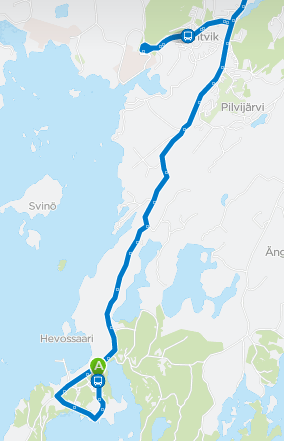
\includegraphics[width=.25\textwidth]{../assets/images/hsl1.png}};
\node at (-1.4, 2.4) {\textbf{(b)}};    

\node (fortum) at (3.5,1)
    {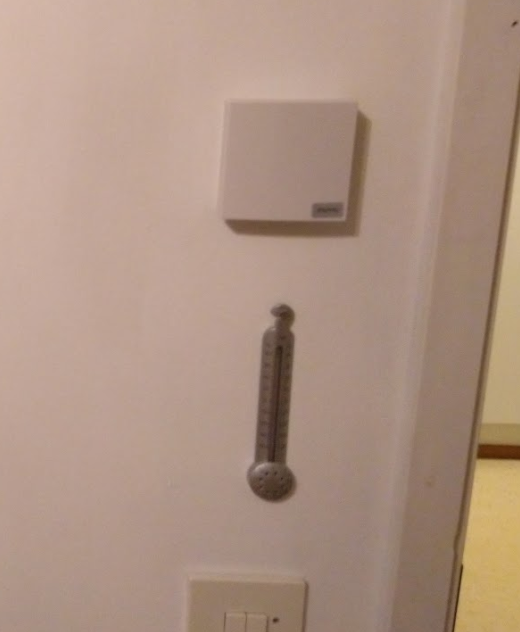
\includegraphics[width=.25\textwidth]{../assets/images/smartliving1.png}};
\node at (2.1, 2.8) {\textbf{(c)}};
\draw [->] (4.5,1) -- (3.7,2);
\node at  (4.5,1) {device};
\node at (-4.5,1.5)
    {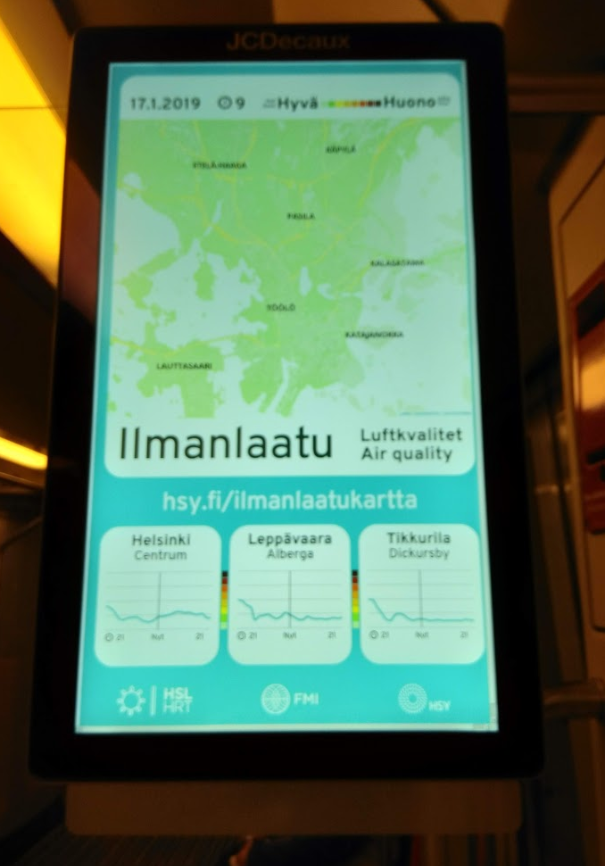
\includegraphics[width=.35\textwidth]{../assets/images/metro.png}};
\node at (-5.8, 4.0) {\textbf{(a)}};

\end{tikzpicture}
\caption{IoT use-cases around us: \textbf{(a)} Screen in the metro wagon showing air quality report in Helsinki metropolitan area. \textbf{(b)} Tracking of a bus in real-time. Service provided by HSL. \textbf{(c)} Devices installed by Fortum as part of their SmartLiving program, in apartment houses in the city of Espoo Finland.  }\label{fig:iot_in_our_lifes}
\end{figure}

One example of IIoT is open data access provided by Finnish national electricity transmission grid operator FINGRID. Near real-time time grid operation measurements are available in machine readable form. The list is too long to list all available data, here we mention just two representative examples: frequency of the power system, power production from different source of energy like nuclear or hydro\footnote{Open data sets and APIs are available at \url{https://data.fingrid.fi/en/}}.  

Above real-world examples, that are in common use today, are all about collecting and presenting data from sensors connected to the Internet. But, as it was mentioned previously, IoT is not just a platform to collect and visualize datafrom different sources. It is also about, of what to do with the collected data, extracting valuable information out of it, using sensors measurements to achieve some goal and many other things that are presented in the list above. Every example of the use case provided is prefixed with word smart, hinting that IoT systems are expected to be embedded with intelligence. 


\subsection{Artificial Intelligence in IoT}
One easy to understand application of artificial intelligence in IoT is Machine Learning (ML) applied to automated data analysis, also known under the name of data mining or big data. A challenging problem, that has a potential to be solved by IoT machine learning is collection of of heterogeneous data from many different sensors and devices, all connected to the same global network connectivity infrastructure, turning data into valuable information from which long-term knowledge and proactive decision making can be deduced. 


Until recently, the state-of-the-art approach of doing IoT machine learning was to collect data from the IoT devices, froward it and process it in the central cloud, either real-time or after data is collected. In other words, performing ML model training, historical analytics or real-time analytics in the cloud where data and compute power are highly available and distributed over many nodes. From the need to handle these large amount of data, not always produced by IoT devices, emerged software for doing computation in such distributed systems like Hadoop and Spark and later
followed extensions to those systems that enable applying machine learning in these highly distributed environments. It was realized that this approach is not scalable and not applicable for use cases where data-privacy, real-time actuation response, intermittent connectivity to cloud, bandwidth constrained data transport, are to be considered. Autonomous car would not send data to cloud for processing to decide does it see a red light or not, the latency is simply too high and will not allow making a timely decision regardless of the connection quality to the cloud. Also, it would not  make sense to send all of the telemetry data generated by the car without any preprocessing, the volume is simply too great, and the value of sending all the data is usually not enough to justify bandwidth and storage capacity usage. That is the reason of why the current state-of-the-art in IoT machine learning is to combine massive capabilities of the cloud with the ability to preprocess the data already in the edge devices, IoT things or do the inference based on the measurements locally.  It might also be the case that security concerns or national regulation prohibit sending data for processing and storage to a cloud, hence making edge processing the most acceptable option.~\cite{stolpe2016internet} 

The data analysis applications, that are using machine learning techniques, are usually trained in the cloud or in the local computing infrastructure of developers and data scientists. After training and tuning process the application is deployed to production environment, meaning edge device or a cloud compute instance using cloud-based management system or by some other means, for example integrating machine learning code into application code. If the machine learning solution is deployed locally on the device, the loose of connectivity to the cloud shouldn't affect the system running on the edge device. The solution must function fully autonomously. There are already products on the market that provide this kind of IoT platform, Amazon AWS Greengrass being one of the most feature complete at the moment.

How to distribute the intelligence so that it can be implemented in one environment and then deployed to various other environments is import subject that we will study in this thesis.

\subsection{Goals and Scope of the Thesis}
In this thesis the deployment of trained machine learning models to IoT devices is explored. IoT devices that are considered here are at least capable of executing Linux operating system. An example of such a device might be a mobile phone, IoT board with Intel processor for embedded applications or even a personal computer.

A prototype application was developed, in an attempt to decouple the code responsible for application logic like user interface from implementation of intelligence. The work is based on the concept of Intelligence Layer (IL) framework proposed in~\cite{edgar2019}. The prototype is called intelligence layer service. One of the tasks of intelligence layer, as presented in~\cite{edgar2019}, is to provide intelligence as a local service to the applications that need it. The concept of IL is not restricted to just being a platform for serving intelligence to client applications, but in this thesis machine learning models description and serving aspects of IL framework are explored. 

ML models are assumed to be mathematical functions. Training of a ML model refers to executing computational algorithm on training data in order to select the most optimal function for a particular problem. 

Decoupled ML model can be represented by a programming code in the form of a library or package for some specific programming language. Other approach is to have a compute instance in a central cloud, executing model on HTTP request from the client program and replying with execution result. Third option is to use Intermediate Representation (IR) format to represent a ML model. Special service will read a model file, turn it into runnable code and expose it to client processes via some Interprocess Communication Protocol (IPC). In this work the third approach is explored. 
        
Intermediate Representation (IR) format describes machine learning model in a library and platform independent way. Two state-of-the-art platform-independent model description formats are presented in Chapter~\ref{chapter:ml_practical}. One of them is used for the IL service prototype.    

The main benefits from decoupling the intelligence from application using IR format, is to allow machine learning solution providers and data scientists, to use any existing machine learning library, that supports the distribution format, to develop their models and deploy them in various kinds of environments.

ML models, produced by different makers and exported to a widely supported IR format, can be translated to IR format and published in a model market or repository. 

Users wanting to integrate the intelligence into their IoT environment production code, will be able to buy and download the model and use it in their IoT environment to perform intelligent tasks. The user can use any machine learning library or runtime that has a backend to translate IR into library's or runtime's native format or executable machine code for a target device. This will allow the user to choose the computation platform that is most suitable for his task and compute requirements.

This approach has also a potential to make a deployment of machine learning models easier and democratize the machine learning space by not bounding model producers and consumers into specific libraries, runtimes or cloud services. The approach can also allow model user to switch between different models and model providers if they choose to do so, without major changes to their code.

The major contribution and goal of this work is to study the possibility of decoupling the intelligence from application and research state of the art solution that enable this decoupling.

\subsection{Structure of the thesis}
\textbf{Chapter}~\ref{chapter:ml_theory} and \textbf{Chapter}~\ref{chapter:ml_practical} provide a general background information related to machine learning. \textbf{Chapter} ~\ref{chapter:ml_theory} covers the theory behind artificial intelligence and machine learning. It also has as subsection covering the most frequently used machine learning models in IoT data analyzing applications.

 \textbf{Chapter}~\ref{chapter:ml_practical} presents practical aspects of machine learning like what state-of-the-art libraries are used to create machine learning applications and current state-of-the-art formats for distributing machine learning models. Some examples are provided showing how machine learning code, for simple ML problems, looks like. It is assumed that reader is relatively familiar with \texttt{Python} and \texttt{C++} programming language and examples are not explained in detail.  

\textbf{Chapter}~\ref{chapter:implementation} describes a prototype implementation of IL machine learning model serving concept. The software architecture of the IL service  implementation is presented and implementation details of the architecture are explained.

In \textbf{Chapter}~\ref{chaper:results} results are described. In that chapter a quick comparison between PMML and ONNX is provided and motivation for using ONNX as a model format is explained. In the chapter it is also explained how ONNX model must to be modified in order to prepare it for successful provisioning to IL.           

\clearpage
\section{Machine Intelligence and Machine Learning}\label{chapter:ml_theory}
Machine learning is a subset of AI techniques and methods for building artificially intelligent systems~\cite{Jung2018}. In recent years, one particular class of function-based machine learning methods called deep learning was used successfully to solve artificial intelligence tasks that were difficult to solve using classical function-based machine learning techniques or other traditional model-based AI methods like rule based- or represent-and-reason methods~\cite{Goodfellow-et-al-2016, Darwiche17}. Solutions to problems related to object recognition and localization in images or natural speech recognition were improved significantly by applying deep learning techniques, and new applications in different domains emerge all the time~\cite{lecun2015deep}. Even more impressive are combination of model- and function-based techniques as shown by current artificial champion AlphaGo in the game of Go~\cite{Darwiche17, silver2017mastering}. These recent advances in AI created a lot of interest in general public outside the scientific community, in research community, industry and government to apply machine learning and AI to various application domains. 

In this chapter we will consider fundamental ideas related to artificial intelligence and machine learning. First, we will consider the concepts of machine intelligence and intelligent agent. After that, we will present how to formally specify machine learning problem and present some classical machine learning models and basic building blocks of a deep learning models.       
\subsection{Machine Intelligence}
The original big goal of AI was to create a machine that is capable of achieving human level of intelligence, reaching the human’s level of performance in cognitive tasks~\cite{Darwiche17}. \textbf{Machine Intelligence (MI) is limited AI}. The objective of MI is not to reach human level of intelligence, but to solve tasks that are considered intelligent. Classifying a piece of text as a funny story can be considered as machine intelligence. Many order of magnitude more difficult task, for a machine, of writing a funny story is outside of the scope of machine intelligence. Automation of tasks currently done by humans like controlling a vehicle in the real-world environment or doing customer support via phone or chat are also examples of domains where machine intelligence is in the process of being applied or is already applied~\cite{BojarskiCars16}. 

It is not easy to define machine intelligence precisely because definition of intelligence itself is difficult. The Oxford English Dictionary defines intelligence as a faculty of understanding. The word faculty, in the context of intelligence, means natural or acquired ability to do something. Expanding the definition by including meaning of faculty we get:

\begin{center}
\textbf{Intelligence} is natural or acquired ability to understand.
\end{center}

If in front of the definition above we add word machine, then it is better to replace word natural with intrinsic. There is nothing natural in computer program or current state-of-the-art electronic computing hardware created by humans. We understand natural as something created by nature. Things created by humans are artificial.    

Living beings act based on their reflexes and understanding to survive, spread and achieve some objectives and machines can be programmed to do the same. Based on presented chain of reasoning the machine intelligence can be defined as:

\begin{center}
\textbf{Machine Intelligence} is an intrinsic or acquired ability of a computing machine or a computer program to understand and carry out actions to achieve objectives and goals of its creator.
\end{center}

In our work we consider creator to be a person or a group of people that designed and implemented machine intelligence. The intrinsic ability might be represented by a model or function suitable for specific problem. Acquiring ability to understand is learning. Learning might represent fitting a curve to available training data or finding model parameters. The learned model can be used to perform an intelligent task. 

The notion of intelligent agent is fundamental and useful mental tool for analysing and designing systems with machine intelligence capability~\cite{AIMA}. Next subsection explains the notion.    

\subsection{Intelligent Agents}
The term agent is used in many closely related areas of science and technology but doesn't have a single universally accepted definition~\cite{wooldridge_jennings94}. In~\cite{wooldridge_jennings94} two views of agency are presented: a weak notion and a strong notion.

In a weak notion of agency, the agent is a software process or a combination of software and hardware that has the following four properties~\cite{wooldridge_jennings94}:

\begin{enumerate}
\item
Autonomy: agents have control of their internal states and actions and can operate without external interaction by other agents or humans.
\item
Social ability: agents are capable of communicating with each other using some common communication protocol 
\item
Reactivity: ability to understand their environment and ability to react to changes in the environment
\item
Pro-activeness: Agent can take an initiative and act preventively in order to achieve their goals
\end{enumerate}

For a stronger notion of agency, in addition to the properties from the weaker notion, agent is represented using concepts more applied to humans like knowledge, believe, desire and intention~\cite{wooldridge_jennings94}. The stronger notion of agency is nearer to the big goal of AI as it was presented in the introduction to this chapter. Hence, for this thesis weaker notion of agency provides suitable scope for the work.

One other important property that is treated in the context of agent systems is rationality~\cite{wooldridge_jennings94}. In popular university text book~\cite{AIMA} on AI by Russell and Norvig, authors base their presentation of AI systems on the notion of rational agent. The general definition of an agent in~\cite{AIMA} coincide with weaker notion of agency presented in~\cite{wooldridge_jennings94}. According to~\cite{AIMA}  agent is expected to: act autonomously, apprehend their environment, maintain persistency over its lifespan, adjust its behaviour according to changes in the environment, create and achieve goals. The rational agent is an agent as described in the previous sentence that acts to achieve its objective as well as possible~\cite{AIMA}. 

In~\cite{Jung2018} instead of the agent the concept of artificial intelligent system that act rationally is used. The system is rational if as a result of interaction with its environment it can take actions to maximize a long-term return.

In the description of an intelligent agent we used general concept like: actions, interaction, communication, environment, goals, objectives, long-term return. It is important to understand that when we talk generally about these concepts there is a lack of concreteness. When the real machine intelligence problem is considered all these concepts become very concrete. Let's consider an imaginary problem from domain of predictive maintenance in petroleum industry related to transporting gas over the pipelines lying deep on the seabed. The task might be to predict leaks in pipes and malfunctions in the gas pumping equipment to prevent natural disasters or to achieve a continuous operation and delivery. The environment is sea, pipes, gas, equipment that enables operation of the whole system. The long-term objective of the agent is to prevent natural disasters and maximize continuous delivery of gas. The agent perceives the environment via the network of sensors scattered over gas delivery system. Action of agent is to communicate to the human operator via computer screen or other digital means of communication that there is a high probability of an emergency situation. One other possibility is to place intermediate agents between agent that detect anomalies and human operators. One intermediate agent might suggest the optimal set of action that might trigger actions of the other agent that is a robot. The robot will go on-site to gather more information so that human operator can choose the best series of actions to maximize performance or mitigate the risks in timely manner. The agents must have a common protocol to communicate with each other and human operator.

The main task of rational agent is to map precept sequence to action that effect environment in a way that maximizes performance measure. The percept sequences are obtained from sensors and actions are applied to environment via actuators. Agent is described mathematically via agent function. Agent function is mapping from a set of percept sequence $S$ to a set of actions $A$:
\begin{align*}
f:S \rightarrow A
\end{align*}

The actuators and sensors are not necessary things that effect physical world directly. They might be buffers in computer memory or sockets in the network connection. The full description of performance measure, environment, actuators and sensors is called task environment. The machine intelligence problem is usually approached by first specifying task environment. The software implementation of agent function is called agent program. The computing devices with sensors, actuators and system level software that form and execution environment for an agent program is called architecture.~\cite{AIMA}   

Currently the preferred method for creating agents is to create a learning agent~\cite{AIMA}. One might even consider saying that it is impossible to implement machine intelligence systems in complex task environment without machine learning~\cite{Jung2018}.         

\subsection{Machine Learning}
Machine learning is mostly concerned with fitting a mathematical model to data and improving the model over-time using the observed evidence from the new data. Every component of an intelligent agent can be improved or implemented by using machine learning techniques~\cite{AIMA}. The model might be represented by a function mapping inputs to outputs. In the introduction to this chapter, we named this approach the function-based machine learning. On the other hand, the model might contain some prior knowledge about the environment represented by probability distributions or general first-order logic. Probability theory and first-order logic are formal languages for describing environments. Machine learning techniques that utilize these formalisms are called model-based machine learning techniques.~\cite{Jung2018, AIMA, Darwiche17} In this thesis only function-based machine learning models are considered. For a complete review of function- and model-based ML models reader can refer to classical text on AI like~\cite{AIMA} by Russell and Norvig.

There are three principal types of machine learning: supervised, unsupervised and reinforcement~\cite{AIMA}. The difference is best understood by considering three components that are required to formally specify the ML problem~\cite{Jung2018}. These components are:
\begin{enumerate}
\item
Raw data points, features extracted from raw data points and labels related to data points.
\item 
Hypothesis space.
\item
Loss function.
\end{enumerate}

Data points are raw data precepted by an agent utilizing its sensors. We denote the set containing all possible values that can be assumed by a data point $\mathbf{z}$ by letter $\mathcal{Z}$. The labels are answers to questions or predictions that we want our model to output, domain of all labels $\mathbf{y}$, sometimes word target is used instead of label, is denoted by $\mathcal{Y}$. Most often data points are preprocessed before they are given to the model. As result of this preprocessing, data point is transformed into a vector of features $\mathbf{x}$, extracted from the data point. We assign symbol $\mathcal{X}$ to a space of all the possible feature vectors.~\cite{Jung2018} Using the mathematical notation, we can represent the mapping for data points to labels with the following mapping:

\begin{align}\label{eq:1}
f: \mathcal{Z} \rightarrow \mathcal{Y}
\end{align}

What is referred to as a model is usually a mapping $m:\mathcal{X} \rightarrow \mathcal{Y}$ so we can rewrite  $f$ in \ref{eq:1} as $f = f_{\mathbf{x}} \circ m$ where mapping $f_{\mathbf{x}}:\mathcal{Z} \rightarrow \mathcal{X}$ is a feature vector extractor.
\pagebreak

The hypothesis space $\mathcal{H}$  is a set of all computationally feasible models that we are considering as candidates for the final model $m$. Hypothesis $h$, also called predictor map, from $\mathcal{H}$ is usually a mapping from feature space $\mathcal{X}$ to label space $\mathcal{Y}$.~\cite{Jung2018}

\begin{align}\label{eq:2}
\mathcal{H} = \{h^{(i)}:\mathcal{X} \rightarrow \mathcal{Y} : h^{(i)} \mkern3mu \text{is computationaly feasible} \}
\end{align}

In order to choose an optimal hypothesis $h$, that will be our final model $m$, from hypothesis space \ref{eq:2} we need a measure of how good the model is performing, does it produce correct predictions. The goodness of a hypothesis is evaluated using loss function $l$ \ref{eq:3}. The loss function is mapping from set-cross product of sets $\mathcal{X}$, $\mathcal{Y}$, $\mathcal{H}$ to real numbers. The hypothesis $h$ that minimizes the average loss function is considered optimal and it is chosen as final model $m$ to make inferences.  

\begin{align}\label{eq:3}
l:\mathcal{X} \times \mathcal{Y} \times \mathcal{H} \rightarrow R  
\end{align}

In \textbf{supervised} learning problems labeled data points $(\mathbf{z}^{(i)},y^{(i)}) \in \mathbb{Z} \subset \mathcal{Z} \times \mathcal{Y}$ are provided by the hypothetical teacher. These labeled data points form a numerable training set $\mathbb{Z}$. The job of the model creator is to find the best possible model $m \in H $ that is consistent on training data and generalizes well on new data points that are not in $\mathbb{Z}$. Model is said to be consistent if it achieves near 100\% accuracy over the training set. Usually, it is not possible to achieve 100\% consistency and get high prediction accuracy on new unseen data points. If the model is predicting accurately labels for data points that it has not used for training, it is said to generalize well to new data. If the model is consistent but does not generalize well to new data, it is said that it suffers from overfitting.

In \textbf{unsupervised} learning, only data points are provided $\mathbf{z} \in \mathbb{Z} \subset \mathcal{Z}$. There are no labeled data points available. The job of the model is to group the data points based on some metric of similarity. Unsupervised learning can be considered as assigning hidden labels to data points. Again, we have some hypothesis spaces that group the data points and we try to find optimal hypothesis or grouping.

In \textbf{reinforcement} learning, model or agent learns by receiving reinforcements from the environment. Unlike in supervised learning, there is not teacher that provides the model with correct labels. Based on the input received from the environment model must decide how it should adjust itself in order to improve the performance. AlphaGo, current artificial champion in the game of Go, is an example of applying reinforcement learning problem to solve real world problem~\cite{silver2017mastering}. No human was able to beat the AlphaGo to date. In this thesis will only examine supervised and unsupervised learning models.     

Inputs and outputs of a model can be represented by \textbf{quantitative} or \textbf{qualitative} variables. Quantitative variables are measurable quantities represented by real numbers like pressure, voltage or velocity vector of a point. Note that quantitative variables are not necessary scalars. Velocity vector of a point in an open space is represented by three real number. Qualitative variables take values from a finite countable set of distinct elements. Elements of the set define categories. For that reason, qualitative variables are also called \textbf{categorical}. An example might be a set of integer number from 0 to 9 representing decimal digits. The models that have categorical labels are called classifiers and the models with quantitative labels are regression models or predictors. Models that have both types of outputs are called mixed models~\cite{Jung2018}. 

For some machine learning classification problems that have by definition discreate label space the hypothesis space might contain mapping that map input to continuous variable. The final prediction is then made using a \textbf{decision function} that maps the values returned by hypothesis to labels. If $d$ is decision function we can rewrite $f$ from \ref{eq:1} as mapping composition:

\begin{align*}
f = f_{\mathbf{x}} \circ m \circ d
\end{align*}

One more distinction exists between the machine learning models. They can be \textbf{parametric} or \textbf{non-parametric}. Parametric models are described using a finite set of parameters. For example, if we are predicting scalar value with the model that is represented by polynomial function then coefficients are parameters. Knowing the coefficients, we can calculate prediction.  Non-parametric models use feature vectors obtained from the data points to do prediction or classification.  

The loss function~\ref{eq:3} averaged over available feature vectors from $\mathbb{X}$ is called \textbf{empirical risk}, where $\mathbb{X}$ is defined by:

\begin{align}\label{eq:4}
\mathbb{X} =  \{ (f_{\mathbf{x}}(\mathbf{z}^{(i)}), y^{(i)})|\quad (\mathbf{z}^{(i)},y^{(i)}) \in \mathbb{Z} \}
\end{align}

The empirical risk is usually defined so that the main objective of machine learning algorithm is to minimize the risk. In mathematical terms empirical risk is a high dimensional function and an optimization problem is to find the best possible function from the hypothesis space given observed data that produces the global or local minimum of the high dimensional empirical risk function.            

Now that we have presented basic theory of ML we will consider some common machine learning models used in IoT domain.            

\subsection{Machine Learning in IoT domain}\label{sec:ml_in_iot}
The major use of machine learning in IoT domain is data analytics. In~\cite{mahdavinejad2017machine} an extensive evaluation and literature review of most frequently used machine learning techniques applied to data produced in the smart city environment was conducted. The result of this work is presented in Table \ref{tab:common_model_iot}. The table is modified from its original form. As can be seen from the table, most of methods can be used for both classification and regression tasks and there are more supervised than unsupervised methods. This reflects the fact that supervised learning techniques are much more developed than unsupervised methods and are used more in application.   

\begin{table}[h!]
\caption{Common machine learning models for IoT.} \label{tab:common_model_iot}
\begin{center}
\begin{tabular}{ |p{4cm}|p{2.5cm}|p{2.5cm}|p{3.2cm}| } 
\hline
\textbf{Model Name} & \textbf{Type} & \textbf{Usage}  & \textbf{Parametrization} \\
\hline
K-Nearest Neighbors & Supervised & Classification Regression  & Non-parametric \\ 
\hline 
 Naïve Bayes & Supervised & Classification & Parametric \\ 
\hline
Support Vector Machine & Supervised  & Classification Regression & Non-Parametric  \\ 
\hline 
Linear Regression  & Supervised  & Regression & Non-parametric  \\
\hline
Decision Trees  & Supervised  & Classification Regression & Non-parametric \\
\hline
Bagging  & Supervised  & Classification Regression & Depends on the base model  \\ 
\hline
Random Forest  & Supervised  & Classification Regression & Non-parametric   \\
\hline
K-means  & Unsupervised  & Classification & Parametric  \\
\hline
Principal Component Analysis  & Unsupervised  & Dimensionality reduction Feature extraction & Parametric  \\
\hline
Feed Forward Neural Networks  & Supervised Unsupervised  & Classification Regression & Parametric  \\
\hline   
\end{tabular}
\end{center}
\end{table}

The first column of Table~\ref{tab:common_model_iot} describes the name of the model. Second column describes the type of machine learning: supervised or unsupervised. Third column describes is model used for classification or regression tasks. Note that most models can be used of both tasks. Fourth column describes, is the model parametric or non-parametric.
%, or mixed. Mixed means that it depends on parameters and a subset of training data.

For models in Table~\ref{tab:common_model_iot} we present typical feature space, label space and hypothesis space in Table~2. Second column after the name column is for input feature space. Third column describes output label space. Fourth column is a short description of model with mathematical description of its hypothesis space or decision function. Note that dimensions and elements of the spaces are picked randomly. The space of real numbers can be replaced by any other metric space. Metric space is set of elements that have a definition for a measure of distance between any two elements from the set. The hypothesis spaces presented in Table~2 might not match precisely with other formulation provided in the literature. Because neural networks are currently among the most popular machine learning methods, we talk about them in more detail in next subsection and show how the concepts presented in Machine Learning section apply to the most basic type of neural network.      
\newpage
%\begin{table}[h!]
Table 2: Description of common machine learning models from Table~\ref{tab:common_model_iot}.
%\begin{center}
\begin{longtable}{ |p{3cm}|p{1.5cm}|p{2.2cm}|p{9cm}| } 
\hline
\textbf{Model Name} & \textbf{Feature Space} $\mathcal{X}$ & \textbf{Label Space} $\mathcal{Y}$  & \textbf{Description and hypothesis space} \\
\hline
K-Nearest Neighbors \newline Classification 
& $\mathbf{x} \in R^2$ 
& $y \in \{a, b, c\}$ 
& $\hat{y} = h(\mathbf{x}, k, \mathbb{X})$ where is $\hat{y}$ is predicted label, $k$ is number of neighbors and $\mathbb{X}$ is training set with feature vectors extracted from raw data points and labels as defined in~\ref{eq:4}. Using some metric like Euclidean measure, distances between input vector $\mathbf{x}$ and $k$ nearest vectors from $\mathbb{X}$ are calculated and label is assigned using majority vote. For example if $k=3$ and 3 nearest neighbors have labels $a,a,b$ then $\hat{y}=a$.      
\\ 
\hline 
K-Nearest Neighbors \newline Regression 
& $\mathbf{x} \in R^2$ 
& $y \in R$ 
& For regression, label space is continuous and $\hat{y}$ is equal to the mean value calculated from the labels of the k nearest neighboring points from training set $\mathbb{X}$. 
\\
\hline
Naïve Bayes 
& $\mathbf{x} \in R^2$  
& $y \in \{a, b, c\}$ 
& The hypothesis space is parametrized by conditional probability distributions of the elements of feature vector conditioned on the label values and the so called prior probability distribution of labels. The decision function is:

\begin{align*}
\hat{y} = \argmax_{y \in \mathcal{Y}} P(y)P(x_1|y)*P(x_2|y) 
\end{align*}  

The feature vector $\mathbf{x}$ is assumed to be random variable and its elements $x_{1}$ and $x_{2}$ independent random variables. This assumption of independence is the reason why the method is called naive. Prior $P(y)$ is usually estimated by the frequency of occurrence in training set. If size of the training set $\mathbb{X}$ is N and point with label $a$ occurs $n_a$ times in $\mathbb{X}$ then prior $P(a)$ is estimated by $P(a)=\frac{n_a}{N}$. Conditional probability $P(x_i|y)$ is usually estimated by  a probability distribution in the form of a function like Gaussian or exponential probability distribution. The parameters for chosen distribution, like mean and variance are estimated from training data.      
\\ 
\hline 
Support Vector Machine \newline Classification 
& $\mathbf{x} \in R^d$  
& $y \in \{-1, 1\}$
& We provide two class classification problem as an example. This model can be extended to multiple classes using one-versus-rest formulation. The classifier is defined by:

\begin{align*}
h(\mathbf{x})=sgn(\sum_{i}^{n} \alpha_i k(\mathbf{x}^{i}, \mathbf{x}) + b)
\end{align*}

Here $\alpha$ are real numbers solved by the learning algorithm using the training data. $k$ is kernel function defined by:

\begin{align*}
k(\mathbf{x},\mathbf{x}’)= \theta(\mathbf{x}) \cdot \theta(\mathbf{x}’)
\end{align*} 

Where $\theta$ is some vector valued function and $\cdot$ denote vector dot product. Hence the classification function in hypothesis space depend on the choice of $\theta$ and samples from training data. $b$ is bias and $sgn$ signum function that returns $1$ if input is positive number and $-1$ if input is negative number.~\cite{lampert2009kernel}   
\\
\hline
Support Vector Machine \newline Regression
& $\mathbf{x} \in R^d$  
& $y \in R$ 
& The hypothesis space for SVM regressor resembles hypothesis for linear regression with feature vector replaced by $\theta(x)$.
\begin{align*}
h(x) = \mathbf{w} \cdot \theta(x)+ b
\end{align*}
$\mathbf{w}$ vector and intercept $b$ are learned from training data.~\cite{lampert2009kernel}    
\\
\hline
Linear regression  
& $\mathbf{x} \in R^2$  
& $y \in R$
& The most basic technique for machine learning and a text book favorite. The hypothesis is defined by

\begin{align*}
h(\mathbf{x}) = \mathbf{w} \cdot  \mathbf{x} + b = w_{1} x_{1} + w_{2} x_{2} + b
\end{align*}

The model is parametrized by weight vector $w \in R^2$ and intercept $b \in R$. 
\\ 
\hline
Decision Trees \newline Classification \newline Regression
& $\mathbf{x} \in R^2$
& \newline $y \in R$ \newline $y \in \{0,1,2\}$ 
& Decision tree learning algorithm partitions the feature space into non-overlapping subspaces, it stratifies the feature space. For two-dimensional feature space in this example, the partition is easy to visualize with a figure. Figure I. below, shows recursive binary splitting of a feature space restricted to a unit square $[0,1]\times[0,1]$. Points in Figure I. represent samples from the training set. Color and shape of the points represent labels. Red circle is 0, green diamond is 1 and blue square is 2. Areas in each strata form subspaces $R_i$. The splitting lines are defined by values $t_i$.~\cite{john2010elements}
\begin{center}
\tikzstyle{label_0}=[circle, draw,fill=red,minimum size=1.5mm, inner sep=0pt]
\tikzstyle{label_1}=[diamond, draw,fill=green,minimum size=2mm, inner sep=0pt]
\tikzstyle{label_2}=[rectangle, draw,fill=blue,minimum size=1mm, inner sep=0pt]
\begin{tikzpicture}
%\draw[help lines] (0,0) grid (4,4);
%Feature space
\draw (0,0) -- (0,4) -- (4,4) -- (4,0) -- (0,0);

% Data points
\node [label_0] at(0.5,0.5) {};
\node [label_0] at(1,0.5) {};
\node [label_0] at (2.5,0.5) {};
\node [label_0] at (2.5,0.5) {};
\node [label_2] at (3.5,0.5) {};

\node [label_1] at(1,1) {};
\node [label_0] at(1.5,1) {};
\node [label_2] at(2.5,1) {};
\node [label_2] at(3.0,1) {};

\node [label_2] at(2.5,1.5) {};
\node [label_2] at(3.5,1.5) {};

\node [label_1] at(0.5,2.0) {};
\node [label_0] at(1.0,2.0) {};

\node [label_2] at(0.5,2.5) {};
\node [label_2] at(1.0,2.5) {};
\node [label_2] at(1.5,2.5) {};
\node [label_0] at(2.0,2.5) {};
\node [label_1] at(3.0,2.5) {};
\node [label_1] at(3.5,2.5) {};

\node [label_2] at(0.5,3.0) {};
\node [label_2] at(1.0,3.0) {};
\node [label_1] at(1.5,3.0) {};
\node [label_0] at(2.0,3.0) {};
\node [label_0] at(2.5,3.0) {};
\node [label_1] at(3.0,3.0) {};
\node [label_1] at(3.5,3.0) {};

\node [label_2] at(0.5,3.5) {};
\node [label_2] at(1.0,3.5) {};
\node [label_2] at(1.5,3.5) {};
\node [label_0] at(2.0,3.5) {};
\node [label_1] at(3.0,3.5) {};
\node [label_2] at(3.5,3.5) {};

% Splits 
\draw [dashed, thick] (0, 1.6) -- (4, 1.6) ;
\draw [dashed, thick] (1.8, 4) -- (1.8, 1.6) ;
\draw [dashed, thick] (2, 0) -- (2, 1.6) ;
\draw [dashed, thick] (2.7, 4) -- (2.7, 1.6) ;
\node [left] at (0, 1.6) {$t_1$} ;
\node [above] at (1.8, 4) {$t_2$} ;
\node [below] at (2, 0) {$t_3$} ;
\node [above] at (2.7, 4) {$t_4$} ;

% Region labels
\node [below right] at (0, 1.6) {$R_1$} ;
\node [below left] at (4, 1.3) {$R_2$} ;
\node [above left] at (1.8, 1.6) {$R_3$} ;
\node [below left] at (2.7, 4) {$R_4$} ;
\node [above left] at (4, 1.6) {$R_5$} ; 

% Axes labels
\node at (-0.5, 2.0) {$x_2$} ;
\node at (2.0, -0.8) {$x_1$} ;

% Fitted model
\node at (0.6, -0.8) {$c_1=0$} ;
\node at (5, 1) {$c_2=2$} ;
\node at (-1, 3) {$c_3=2$} ;
\node [above]at (1, 4) {$c_4=0$} ;
\node [right]at (4, 3.5) {$c_4=0$} ;

\node at (5,-1) {\textbf{Figure I.}};
\end{tikzpicture}
\end{center}
For each region a simple model is fitted to the data. In the case of regression, it is constant calculated as a mean of all training samples inside the region. For classification decision tree the most dominating label among the training points in the region can be chosen as a label for the whole region. In Figure I classification problem is assumed. The dominating labels are denoted by $c_i$ in the figure.~\cite{john2010elements}    

The hypothesis space is composed of all possible partitions of feature space or its subspace. The hypothesis for the classifier and predictor estimating continues values have identical equations. Equation~\ref{eq:5} depicts hypothesis map for partition presented in Figure I. $I$ is a function that returns $1$ if $\mathbf{x}$ is inside region $R_i$ and $0$ if it doesn't belong to the region.~\cite{john2010elements}

\begin{equation}\label{eq:5}
h(\mathbf{x}) = \sum_{i=1}^{5}c_iI(\mathbf{x} \in R_i)
\end{equation} 
\\
\hline
Decision Trees \newline Classification \newline Regression
& $\mathbf{x} \in R^2$
& \newline $y \in R$ \newline $y \in \{0,1,2\}$
& The decision tree is grown by recursively splitting the features space into non-overlapping regions. The technique is called decision tree because the hypothesis can conveniently be represented by a tree structure.~\cite{john2010elements}              
\\
\hline
Bagging
& 
&  
& Bagging is also referred to as bootstrap aggregation. In bootstrap aggregation the prediction of a hypothesis map of a base model is averaged over a collection of bootstrap samples with goal of reducing the variance of estimation.~\cite{john2010elements}

If there is $M$ bootstrap samples $\mathbb{X}^{*b}$ partitioning the training set $\mathbb{X}$, we fit the base model to each sample getting the optimal base hypothesis map $m^{*b}$. The final prediction is an average over base hypothesis maps~\cite{john2010elements}:
\begin{align*}
h(\mathbf{x})=\frac{1}{M}\sum_{b=1}^{M} m^{*b}(\mathbf{x})
\end{align*}
The above formula is for regression problem. For classification problem for each class indexed by integer $k$ the proportion of models $p_{k}(\mathbf{x})$ predicting class $k$ is calculated for data point $\mathbf{x}$. Bagged classifier returns value that has the highest proportion.~\cite{john2010elements}      
\\
\hline
Random Forest
&
& 
& Random forest model is a modification to bagging with a decision tree as a base predictor. It constructs a large collection of de-correlated trees and then averages the predictions from them to calculate final result like in bagging. The predictor map is similar to what was presented for bagging. The correlation is reduced by random selection of features from a feature vector at each step of growing a regression tree.~\cite{john2010elements}.    
\\ 
\hline
K-Means
& $\mathbf{x} \in R^2$
& $y \in {1,...,k}$
& In k-means machine learning technique the algorithm clusters the points from training set into $k$ clusters, calculating the centroid for each cluster, using some similarity measure to determine which point should belong to same cluster. $k$ is hyper-parameter representing the assumption about the data. For the data points in $R^2$ the similarity might be Euclidean distance or the dot product of two feature vectors. This method doesn't require labeled data. Clustering can be interpreted as extreme case of classification problem when labels for the data points in training set are not available.~\cite{Jung2018}   

The classifier function assigns a label to new input data point based on what centroid is nearest to the data point. The hypothesis space if formed by all possible cluster assignments and the decision functions might be:
\begin{align*}
h(\mathbf{x})=min(\argmin_{y \in \mathcal{Y} }{||\mathbf{x}-m_y||})
\end{align*}
Here, $m_y$ are cluster centers. $min$ functions picks the class with minimal index. If distance between $\mathbf{x}$ and multiple centers is the same and $argmin{||x-m_k||}$ is a set that has more than $1$ element we need strategy to choose only one class, for that $min$ is used.~\cite{Jung2018}       
\\
\hline
Principal Component Analysis
& $\mathbf{x} \in R^{13}$ 
& $\mathbf{y} \in R^2$
& Principal Component Analysis is used to reduce the number of features in the high dimensional feature vector that is fed to machine learning model as input. Using high dimensional feature vectors requires a lot of compute and memory resources to execute the model. For some models using large number of features might produce an overfitting effect. Reducing the number of features to two is sometimes useful to visually inspect data.  For these reasons reducing the number of feature is beneficial.~\cite{Jung2018}

The hypothesis map for PCA is linear transformation define by matrix $\mathbf{W}$. For our example this is $13$ by $2$ matrix. How this matrix is calculated is out of scope for our work. Interested reader can read~\cite{Jung2018} to find out more about PCA.    
\\
\hline
Feed Forward Neural Networks
& $\mathbf{x} \in R^2$
& $\mathbf{x} \in R$
& A type of neural network without feedback loops. The hypothesis space is defined by network topology and a set of numerical parameters. The output of a neural network is usually continuous. For classification problem it can indicate the score or probability of belonging to different classes in a classification problem. Decision function for classification problem picks the class that has highest probability. 

Because of the current popularity of neural networks they will be treated in more detail in Subsection~\ref{sub:nn}.         
\\
\hline   
\end{longtable}
%\end{center}
%\end{table}

\subsection{Neural Networks\label{sub:nn}}
The most fundamental building block of any computational neural network is Rosenblatt's perceptron, named after a psychologist Frank Rosenblatt who published a paper presenting it in 1958. The perceptron represents a single unit of computation, that applies an affine mathematical operation and optional non-linear mathematical function to one or more scalar inputs producing a single scalar output. The perceptron is a single neuron of a neural network, and a neural network is build out of such neurons with connected inputs and outputs.~\cite{haykin2009neural} 
\usetikzlibrary{arrows,decorations.markings}
\begin{figure}[h!]
\centering
\tikzstyle{label_0}=[circle, draw,fill=red,minimum size=1.5mm, inner sep=0pt]
\tikzstyle{label_v}=[circle, draw,fill=red,minimum size=5.0mm, inner sep=0pt]
\begin{tikzpicture}[node distance=1cm]
\node (x1) [label_0] at (0, 2) {};
\node [above left] at (x1) {$x_1$};
\node (x2) [label_0] at (0, 1) {};
\node [above left] at (x2) {$x_2$};

\node at (0,0.5) {$\texttt{.}$};
\node at (0,0) {$\texttt{.}$};
\node at (0,-0.5) {$\texttt{.}$};

\node (xn1)  [label_0] at (0, -1) {};
\node [above left] at (xn1) {$x_{n-1}$};
\node (xn) [label_0] at (0, -2) {};
\node [above left] at (xn) {$x_n$};

\node (v) [label_v] at (4, 0) {$v$};
\node (b) [label_0] at (4, 2) {};
\node     [above] at (b) {$b$};

\node (phi) [label_v] at (7, 0) {$\phi$};
\node (y) [right] at (9, 0) {$y$};

\draw (x1) edge[->,>=stealth] node[above] {$w_1$} (v);
\draw (x2) edge[->,>=stealth] node[below] {$w_2$} (v);

\draw (xn1) edge[->,>=stealth] node[above] {$w_{n-1}$} (v);
\draw (xn) edge[->,>=stealth] node[below] {$w_n$} (v);
\draw (v) edge[->,>=stealth] node[above] {$v=\mathbf{w} \cdot \mathbf{x} +b $} (phi);
\draw (phi) edge[->,>=stealth] node[below] {$\phi(v)$} (y);
\draw (b) edge[->,>=stealth] (v);

\end{tikzpicture}
\caption{Graph diagram of Rosenblatt's perceptron. }\label{fig:graph_perceptron}
\end{figure}

Figure~\ref{fig:graph_perceptron} illustrates Rosenblatt's perceptron as a directed graph. Scalars $x_{i}$, where $x_i \in R$, are inputs and can be thought of as components of $m$-dimensional input vector $\mathbf{x} \in R^{m}$. The directed arrows starting at inputs and converging at a single point are called synapses and a scalar number assigned to each synapse is called a synaptic weight. One other converging arrow with bias value $b$ is not part of the input and is internal to the perceptron, it can be thought of as a translating component of an affine transformation. Using synaptic weights and bias perceptron does affine transformation taking a dot product between input vector $\mathbf{x}$ and a vector of synaptic weights $\mathbf{w}$ and adding bias $b$ to the result. The result of affine operation is called local field $v$. Formula for local $v$ field is:

\begin{align*}
v = \mathbf{w} \cdot \mathbf{x} + b 
\end{align*}

The nonlinear operation can be any real valued function $\phi$ that takes local field as input and produces final output of neuron. $\phi$ is also called activation function. Some choices of activation function where found to be better than others for numerical stability and theoretical inferences like mathematical proofs. In practice only, couple of well-known and well-studied function are used for activation of a neurons. The symbolic mathematical expression for the perceptron is simply:

\begin{align}\label{eq:perceptron}
y = \phi(v) = \phi(\mathbf{w} \cdot \mathbf{x} + b) 
\end{align}

Rosenblatt’s perceptron can be trained to classify a linearly separable pattern in a finite number of steps~\cite{haykin2009neural}. If a feature space is a subspace of $R^2$ and a label space consists of only two labels, that is we are trying to solve a binary classification problem, the pattern is linearly separable if points belonging to different classes can be separated by a line. In higher dimensional space the line is a hyperplane. 

We will now present an example of a perceptron to do binary classification of a linearly separable pattern in two-dimensional feature space to highlight the basic concepts of machine learning presented in previous subsections. We assume that the features are already extracted from the raw data and feature space is $\mathcal{X} = R^2$. Usually the process of identifying how to extract features and what features are import is quite involved process but we skip it here, because it is a very domain specific problem. The label space consists of two number $\mathcal{Y} = \{-1, 1\}$, number $1$ identifies belonging to class $\mathfrak{C_{1}}$ and number $-1$ to class $\mathfrak{C_{2}}$. The model is described by a neuron with two inputs and activation function is an identity. The decision function is a signum function that outputs positive one for positive value produced by a neuron and respectively negative one for negative number. The hypothesis space is parametrized by two weights and a bias values. For that reason, we can identify hypothesis space with $R^3$.  

At this point we have defined: feature space, label space, model, hypothesis space and a decision function. To train the model we still need a loss function, empirical risk and training data. We denote the finite, discreate training set of $N$ training samples by $\mathbb{X}$. Elements of this space are tuples $(\mathbf{x}^{(i)}, y^{(i)})$ where $ \mathbf{x}^{(i)} \in \mathcal{X}$ and $ y^{(i)} \in \mathcal{Y}$. The loss function needs to be small when model classifies input feature vector correctly, indicating the correct prediction and the value of the loss function needs to be large when the model misclassifies the feature vector. For our problem we can use the following loss function $l$:

\begin{align}\label{eq:logistic_loss}
l((\mathbf{x},y),h) = \ln{(1+e^{-yh(\mathbf{x})})}
\end{align}

This function is called logistic loss function. The hypothesis map $h$ is as in expression~\ref{eq:perceptron} with $\phi$ set to identity function. If we fix the value of $y$ to -1 and plot the loss function as function of $h$ we can see the function has large values when $h$ is positive indicating the error in classification and it is decreases rapidly when $h$ has negative values. If $y$ is set to unity the effect is reversed. Plots for both cases are presented in Figure~\ref{fig:logistic_loss}.
 
\usetikzlibrary{datavisualization}
\usetikzlibrary{datavisualization.formats.functions}
\begin{figure}[h!]
\centering
\begin{tikzpicture}
\datavisualization [school book axes, 
visualize as smooth line,
 x axis={label=$h$},
 y axis={label=$l$},
 ]
data [format=function] {
var x : interval [-4:4];
func y = ln(1 + exp(1 * \value x));
}
info {
\node at (4,2) {\textbf{(a)} $l=\ln{(1+e^{h})}$};
};
\end{tikzpicture}

\begin{tikzpicture}
\datavisualization [school book axes, 
visualize as smooth line,
 x axis={label=$h$},
 y axis={label=$l$},
 ]
data [format=function] {
var x : interval [-4:4];
func y = ln(1 + exp(-1 * \value x));
}
info {
\node at (4,2) {\textbf{(b)} $l=\ln{(1+e^{-h})}$};
};
\end{tikzpicture}
\caption{Logistic loss function~\ref{eq:logistic_loss} as a function of $h$  for $y=-1$ in \textbf{(a)} and $y=1$ in \textbf{(b)}.}\label{fig:logistic_loss}
\end{figure}

The empirical risk $\mathtt{EMR}$ is an average of a loss function~\ref{eq:logistic_loss} over all samples from the training set and can be expressed by the formula~\ref{eq:preceptron_emr}. In this formula we have also expanded the mathematical expression showing explicitly dependence of $\mathtt{EMR}$ on elements of weight vector $\mathbf{w}$, bias $b$ and training data from $\mathbb{X}$.

\begin{align}\label{eq:preceptron_emr}
\mathtt{EMR} = \frac{1}{N}\sum_{(\mathbf{x}^{(i)}, y^{(i)}) \in \mathbb{X}}{l((\mathbf{x},y),h)} = \frac{1}{N}\sum_{(\mathbf{x}^{(i)}, y^{(i)}) \in \mathbb{X}}{\ln(1+e^{-y^{(i)} ( \mathbf{w} \cdot \mathbf{x^{(i)}} + b) })} \\= \frac{1}{N}\sum_{(\mathbf{x}^{(i)}, y^{(i)}) \in \mathbb{X}}{\ln(1+e^{-y^{(i)} ( w_1 x_{1}^{(i)} + w_2 x_{2}^{(i)} + b) })}
\end{align}

Now that we have all three components of a machine learning problem we can train the model with the available training data. The loss function~\ref{eq:logistic_loss} we chose has a special property. It is differentiable with respect to hypothesis $h$. Since $h$ is also differentiable with respect to its parameters from the theory of calculus we know that composition or sum of differential function is a differentiable function. We can conclude that loss function~\ref{eq:logistic_loss} and empirical risk~\ref{eq:preceptron_emr} are differentiable functions.                  

By minimizing the empirical risk with respect to parameters we find the best hypothesis that can be used for inference.
The parameters $\mathbf{w}$ and $b$ that minimize empirical risk are the ones that define the hypothesis $m$ that is used to make inferences after training.  Since $\mathtt{EMR}$ is differentiable function we can find a critical point of empirical risk function by equating is partial derivatives to zero as in equation~\ref{eq:pdv}. Critical point can be local/global minimum, maximum or saddle point. Additional investigation must be performed in order find out the type of critical point. For function that are convex, like a parabola in two-dimensional Cartesian real space opening towards positive y-direction, the critical point is minimum but not necessary global minimum.

\begin{align}\label{eq:pdv}
\pdv{\texttt{EMR}}{w_1} = \pdv{\texttt{EMR}}{w_1} = \pdv{\texttt{EMR}}{b} = 0
\end{align}

We presented the most simple type of feed-forward neural network consisting of only single neuron. Neural network used for real world problem are much more complex utilizing other types of neurons that express for example convolution operation. These different types of neurons can form composite block called layer and layers can still be connected further forming very deep topologies. The outer layers are usually referred to as input and output layers, and inner layers are called hidden layer because they are not directly visible to the user of the network. Having many layer is the main reason why neural networks are called deep. Basically any network that has more than one hidden layer is considered deep.  
 
Although in practice networks can be much more complex, as was explained in previous paragraph, they usually are formulated as we have done it for a Rosenblatt’s perceptron. In our example we didn't solve for optimal weights and bias but solution can be found analytically. For complex networks and other types of machine learning algorithms, it is usually near impossible to solve optimization problem of minimizing empirical risk analytically, that is why numerical methods must be used.

If empirical risk is differentiable the most popular methods of solving for optimal values are family of methods based on gradient descent.  Gradient descent method is an iterative algorithm utilizing gradient of empirical risk to iteratively, step by step improve the estimate of a critical point. Gradient is vector field, the values of its components are derivatives taken at some point on the surface of empirical risk with respect to parameters and bias.  Geometrically speaking empirical risk defines a surface in high dimensional space similar to equation of a sphere in 3-dimensional space. Being able to calculate derivatives is critical in utilizing gradient descent method and most of software for creating and training neural networks implement efficient data structures and algorithms for calculating  gradients of complex function representing neural networks.

\newpage
\section{Software Libraries for creating Machine Learning models and Formats for distributing them}\label{chapter:ml_practical} 
In the beginning of this chapter two popular state of the art software libraries for creating, training and executing machine learning algorithms, are presented. After that, we consider two library independent formats for distributing machine learning models. Because of the recent achievements of deep learning models~\cite{tan_lim_2018}, most popular and hyped machine learning libraries are heavily specialized for creating, training and executing, data and compute hungry, deep learning architectures. Most of the libraries are provided as open source software, but behind each popular deep learning library stands on of the industry giants like Facebook, Google or Amazon. There exists quite many deep learning libraries, we mention only a couple: TensorFlow (Google)~\cite{abadi2016tensorflowas}, Caffe2 (Facebook), PyTorch (Facebook)~\cite{paszke2017automatic}, MXNet (Amazon)~\cite{chen2015mxnet} and more exotic based on OCaml functional programming language OWL~\cite{wang2017owl}. One can classify deep learning libraries based on the programming model they provide, to a software developer or data scientist, for defining computations. Currently, two programming models, also word paradigm can be used, exist: declarative approach and imperative approach. In Caffe2 library data scientists can only use the declarative approach. In PyTorch developers can only use the imperative programming model for writing ML code. MXNet supports both paradigms and for that reason we will present it in this chapter, after explaining the meaning and difference between declarative and imperative approaches. We will also present \texttt{Python} scikit-learn library~\cite{pedregosa2011scikit}, the scientific computation environment for doing machine learning and statistics calculations that can be considered a traditional imperative library for doing data-analytics and creating machine learning applications.
Common, to almost all machine learning libraries, is that they are written partially in C, C++ or Fortran\footnote{Mathematical libraries written in Fortran are still used for scientific calculations, especially linear algebra e.g. LAPACK.}, that is so called back-end implementation of the library, for efficiency, but APIs for the users of the library are usually exposed via one or multiple other languages that are considered easier to use. Python being the most popular front-end language at the time of writing this thesis. 

After understanding how ML models are created we will talk about model formats that enable interoperability between different machine learning libraries. Interoperability is to be understood as having a common format for sharing ML models between different ML libraries. Two formats are presented: ONNX~\cite{hazelwood2018applied} and PMML~\cite{guazzelli2009pmml}. The ONNX format will be used as a base for our proof of concept prototype in later chapters of this work.

\subsection{Differences between declarative and imperative approaches}
In most state-of-the-art deep learning libraries, neural networks are represented by Directional Acyclic Graphs (DAGs) also called dataflow graphs. This is done to allow efficient execution of neural network in training and inference and to make possible efficient calculation of partial derivatives by reverse mode algorithmic differentiation. As was described in Chapter~\ref{chapter:ml_theory}, the calculation of partial derivatives is a necessary step for stochastic gradient descent, main technique used for training neural networks and other machine learning models when loss function is differentiable.

In \textbf{declarative approach} to programming deep learning models, the computational graph is defined before any computations take place. After the graph is defined, it is compiled into executable code and then used on every iteration either for inference or training. The graph is \textbf{static}. The declarative approach is also often described as \textbf{define-and-run} method or \textbf{symbolic} approach to machine learning.

\textbf{Imperative approach} can be characterized by the phrase \textbf{define-by-run}, notice the \textbf{by} in the phrase. The graph is constructed \textbf{dynamically} on every iteration. This allows developer to use familiar style of imperative programming for constructing a graph, mixing construction of graph with control constructs of the host programming language like conditionals: \textit{if}, \textit{else} and looping statements: \textit{for}, \textit{while}. It also allows to get intermediate results of calculation much more easier than with declarative approach. The construction of the graph is hidden from the user by the technique called operator overloading that is supported by many popular programming languages e.g. C++ and Python.

The imperative approach is more flexible than symbolic approach. It allows to write and experiment with different deep learning parameter optimization techniques, variation of stochastic gradient descent for example, and network typologies much easier than with rigid static graphs. Declarative approach with static DAG allows for more performant code that can be parallelized and optimized for faster execution much easier than code written with imperative approach hence making training and inference faster. 

Some libraries combine two approaches to benefit from both. For example OWL and MXNet use both techniques. In the code Listings~\ref{listing:declarative} and~\ref{listing:imperative}  we present MXNet code for training a one neuron perceptron classifier with two inputs and with logistic loss function. The code  in Listing~\ref{listing:imperative} is an example of imperative approach. Code in Listing~\ref{listing:declarative} is an example of declarative approach. Code for generating synthetic training data is omitted from the listings.

\lstinputlisting[language=Python,style=protobuf,caption={Declerative MXNet code for training Rosenblatt's preceptron with two synapses, for a binary classification problem using gradient descent method.~\label{listing:declarative}}]{../mxnet/ExamplesForThesis/rosenblatt_perceptron_sym.py}



\subsection{MXNet}
MXNet is a library for creating large-scale deep neural networks. It is possible to do general mathematical computation with MXNet, but the library was designed to help developers to utilize the full computational capabilities of multiple GPUs and cloud compute infrastructure for creating neural networks. After-all Amazon is the main stakeholder for the project. Library offers device placement to allow the developers to easily specify in what memory, data structure used in computations are stored. For example, if computations are executed on the GPU then data structures must be in GPU’s memory and amount of copying between main memory and GPU memory must be minimal to avoid high latency when chucks of memory are moved via slow external buses\footnote{External to CPU cache, GPU memory and main memory. That is buses that allow to move between these devices.}.  It is possible to scale computation over multiple GPUs or network clusters. Library provides automatic differentiation for calculating derivatives to optimize neural networks parameters. Optimized for speed, predefined neural network layers can help developer to create efficient deep neural networks out of the ready-made building blocks without the need to write code for implementing common layers of neural network like fully connected layer where each neuron has a synaptic connections to all outputs of a previous layer of neural network to which it belongs.

\lstinputlisting[language=Python,style=protobuf, caption={Imperative MXNet code for training Rosenblatt's preceptron with two synapses for a binary classification problem using gradient descent method.\label{listing:imperative}}]{../mxnet/ExamplesForThesis/rosenblatt_perceptron_imp.py}

\subsubsection{MXNet Model Server}
The implementation of intelligence layer that we will be present in Chapter~\ref{chapter:implementation} will be used to server ML models locally using some local inter process communication protocol that enables communication between IL and applications that request intelligent services. MXNet Model Server is part of the Apache MXNet project and is software for serving machine learning models using HTTP endpoints as transport protocol. Hence MXNet model server provides functionality that might seem similar to IL at first. But there are some differences.

MXNet model server is oriented more towards cloud environment compared to IL that is supposed to run on device and utilize cloud service as extra functionality. The way how models are provisioned, in the implementation of IL that is presented in this work, are also very different. In MXNet model server, a model that is executed, is represented by a \texttt{Python} program. Allowing for a lot of flexibility in terms of data post- and pre-processing and libraries used to do inference. These approach adds work for intelligence model provider to write additional code around the machine learning model. Implementation of intelligence layer in this work will expect just an ONNX model file that is produced as an artefact during model training and development process.            

It must be reminded to the reader that IL is not just about model serving~\cite{edgar2019}. But in this thesis we only consider the model serving aspects of IL.  
\subsection{Scikit-learn}
In the data science and machine learning community scikit-learn machine learning library is considered rightly an entry point into the science of data analysis and machine learning, because of its nice API design~\cite{buitinck2013api} and very comprehensive documentation.~\cite{pedregosa2011scikit} In contrast to MXNet, scikit-learn has implementation for many different classical machine learning models and its domain is medium-scale learning. Scikit-learn is a \texttt{Python} library and it uses Numpy pckages’s \texttt{ndarray} for representing low and high dimensional mathematical objects like scalars, vectors, matrices and tensors. These two facts make the library beginner friendly and lower the entry barrier into the machine learning world. In this subsection we will highlight the main features of scikit-learn without considering its details. Only one example of very simple application will be provided. The interested reader can refer to extensive scikit-learn’s online documentation to get more informative overview of the library.

The scikit-learn library supports supervised, unsupervised classical machine learning models like generalized linear models, decision trees, support vector machines, clustering, gaussian mixture models, fully connected multi-layer perceptron and many more other models. It also supports model selection and validation techniques like different metrics to evaluate model performance e.g. least mean square measure and cross validation like k-fold cross validation. The transformation of the data like dimensionality reduction or normalization are supported as well.

The main conceptual object of the scikit-learn library is an estimator. Estimators are objects that can be trained from the data and used for predictions. Estimators usually have \textit{fit} method. For supervised learning the parameters to the \textit{fit} method are an array of data points and array of labels that correspond to the data points. For unsupervised learning estimators, only data points are provided. Most of estimators have \textit{predict} and \textit{score} methods to generalize to new data points and evaluate performance of the model. Transformers like PCA have \textit{transform} method to transform the data. Transformers and estimators can be combined a composite estimator by Pipeline objects.

The code in Listing~\ref{listing:scikit_learn_exmp} presents a simple machine learning application that is used to predict the price of one crypto-currency based on the price of other crypto currency using linear regression model. The machine learning algorithm is represented by a pipeline that first uses transformer to standardize, scale and move all the points so that the mean and variance of the input data is $0$ and $1$ respectively, and then applies linear regression to data. Part of the data is used for training and part for testing the model. Note that label data is also standardized. 

\lstinputlisting[language=protobuf3,style=protobuf, caption={Python code, showing how scikit-learn library can be used to train linear model to predict closing price of Etherium crypto-currency based on the closing price of Bitcoin crypto-currency.}\label{listing:scikit_learn_exmp}]{../onnx_experiments/python_examples/scikit_learn_exmp_2.py}

Scikit-learn has a very well designed APIs. It is reasonable to use Scikit-learn's API as and motivating example for designing APIs for model serving solutions like IL. 
    
\subsection{Formats for representing machine learning functions and models} 
Machine learning libraries usually use their own internal data structures to represent calculations or even multiple different data structures suitable for each machine learning technique. These structures are usually expressed by Domain Specific Languages (DSL) or native Intermediate Representations (IR) specific to a library. Different libraries might also support different programming languages for creating machine learning applications. The environment where ML model is developed and trained and where it is supposed to be executed might be drastically different. The image recognition model might be developed and trained in the cloud where computational resource can be acquired on demand. But the deployment environment, where inference on local data is performed, for the same image recognition model might be a mobile phone or IoT device like Raspberry Pi. These facts make it difficult to share models between different libraries and deploy and integrate machine learning solutions into production quality applications. 

It is important from performance and interoperability perspective to be able to develop ML algorithms using one library and then execute or improve it using another library. This requires having a common standardized IR for representing ML models. ML library providers can use this common IR to write converters and backends to enable interoperability with other frameworks. The job of the converter is to translate from the library's native IR to standardized open IR. Backend is supposed to be able to read the model description in standardized IR and execute it or provide the access to native IR format if the purpose is to improve the model by training on different data or evaluating its performance. The standardized IR for ML model might also be considered as standard that enables distribution of machine learning. The aspect of distribution of machine learning is a key aspect of this thesis.

In this section we consider two IR formats. Those formats are listed in the list below. Both of these formats are open. ONNX uses protocol buffers to define the format  and encode the models. PMML is based on XML. The model expressed with ONNX is distributed as protocol buffer file and PMML model is distributed as an XML file. Based on our study of these formats we will pick one as base for our prototype of intelligence layer.

\begin{itemize}
\item
Open Neural Network Exchange (ONNX) format
\item
Predictive Model Markup Language (PMML) format
\end{itemize}

\subsubsection{Protocol buffers}
The Extensible Markup Language XML format used for representing PMML models is a very common encoding for documents and data structures that is human readable and machine readable. We will not cover it in this thesis. Readers who are not familiar with XML can refer to~\cite{bray2008extensible} for more information about XML. Protocol buffers are less well known. We will explain what protocol buffers are in this subsection.

Protocol Buffer (PB) is an alternative format to XML overcoming some of its shortcomings. Protocol buffer was developed internally by Google and made available for general use as an open source project.~\cite{kaur2010evaluation} On the protocol buffer's project web page, PB is described as:

\begin{center}
Language-, platform-neutral extensible mechanism for serializing structured data that is faster, smaller and simpler than XML.
\end{center}

PB is format for serializing and deserializing data structures. It is used in communication protocols, data storage and for other things. Our use case being: representing machine learning models. The data structures are defined in the text files postfixed with \texttt{proto} or \texttt{proto3} postfixes. The \texttt{proto} file contains message types. The messages define structure of the data we want to serialize. Each message has a type and is defined by numbered name-value pairs, as shown in code Listing~\ref{listing:pn_example}. Value type can be integer, floating-point, boolean, string, enumeration, raw bytes or other messages. The name-value pair can have a qualifier in front: required, optional or repeated. The required are required for a message to be valid. Optional fields are as a name suggested optional. Repeated fields are kind of arrays. The message can have zero or one repeated fields. There are two version of protocol buffer language used to define messages, that is reason to have 3 in the proto3 prefix. The full description of PB language can be found online at~\cite{pb_reference}. 

\lstinputlisting[language=protobuf3,style=protobuf, caption={Snippet from protocol buffer definition of a ONNX Tensor. Used to show basic constructs of PB message definition.~\label{listing:pn_example}} ]{assets/pb/example.proto3}

As depicted in Figure~\ref{fig:proto_compile} the messages definitions file is compiled into language specific classes that can be used to serialize and deserialize data in the variety of data streams. Protocol buffer supports many languages: C++, Python, Java and others. That is, it provides compiler to compile proto files and produce native code for all these languages.

\begin{figure}[h!]
\centering
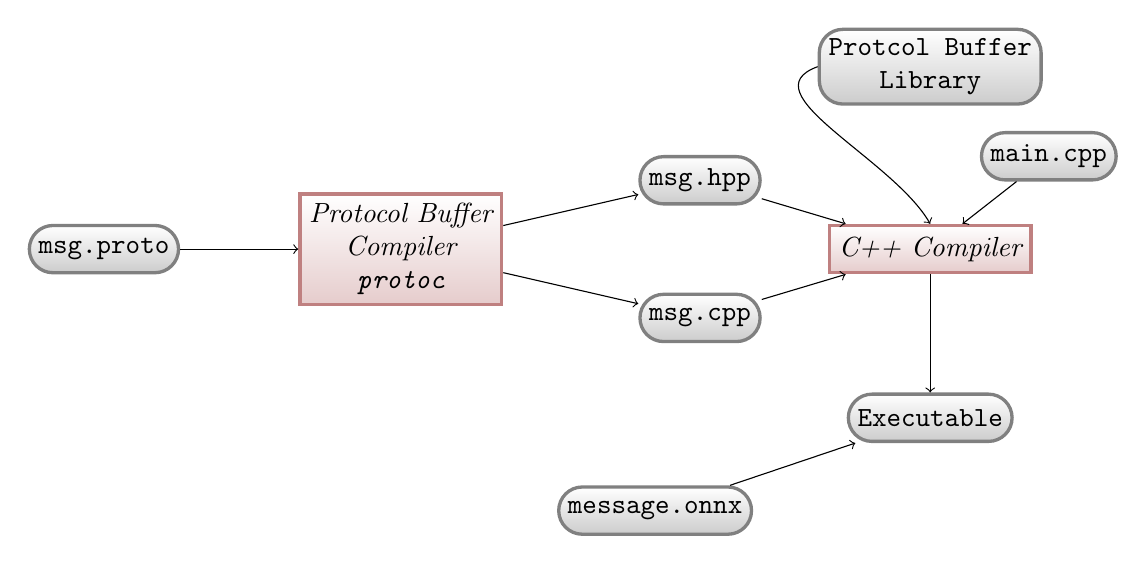
\begin{tikzpicture}[node distance=15mm,
compiler/.style={
% The shape:
rectangle,
% The size:
minimum size=6mm,
% The border:
very thick,
draw=red!50!black!50, % 50% red and 50% black,
% and that mixed with 50% white
% The filling:
top color=white, % a shading that is white at the top...
bottom color=red!50!black!20, % and something else at the bottom
% Font
font=\itshape
},
 file/.style={
% The shape:
rectangle,minimum size=6mm,rounded corners=3mm,
% The rest
very thick,draw=black!50,
top color=white,bottom color=black!20,
font=\ttfamily},
dbus/.style={
% The shape:
rectangle,
% The size:
minimum size=6mm,
% The border:
very thick,
draw=blue!50!black!50, % 50% red and 50% black,
% and that mixed with 50% white
% The filling:
top color=white, % a shading that is white at the top...
bottom color=red!50!black!20, % and something else at the bottom
% Font
font=\itshape
}]

\node (pf) [file, align=center] {msg.proto};
\node (protoc) [compiler, align=center, right=of pf] {Protocol Buffer\\ Compiler \\ \texttt{protoc}};
\node (cp1) [right=of protoc] {};
\node (cp2) [right=of cp1] {};
\node (cp) at ($(cp1)!0.5!(cp2)$) {};
\node (cp3) [above=of cp] {};
\node (cp4) [below=of cp] {};
\node (cpph) [file] at ($(cp)!0.5!(cp3)$)  {msg.hpp};
\node (cppc) [file] at ($(cp)!0.5!(cp4)$)  {msg.cpp};
\node (cc) [compiler, right=of cp] {C++ Compiler};
\node (plib) [file, above=of cc, align=center] {Protcol Buffer\\Library};
\node (prg) [file, below=of cc, align=center] {Executable};
\node (main) [file, below=of cc, align=center] at (12,3) {main.cpp}; 
\node (msgfile) [file, below=of cc, align=center] at (7,-1.5) {message.onnx}; 

\path (pf) edge[->] (protoc);
\path (protoc) edge[->] (cpph);
\path (protoc) edge[->] (cppc);
\path (cpph) edge[->] (cc);
\path (cppc) edge[->] (cc);
\path (cc) edge[->] (prg);
\draw [->] (plib.west) to[out=200,in=120] (cc.north);
\path (main) edge[->] (cc);
\path (msgfile) edge[->] (prg);
%\node (cppc) at ($(fs)!0.5!(dbusio)$) {message.cpp};
%\node (mm) [actor, align=center, below=of md] {Model \\ Manager};
%\node (dbusio) [actor, align=center, right=of mm] {dbusio};
%\node (dots) [below=of mm ] {\texttt{...}};
%\node (ex1) [actor, left=of dots ] {executor};
%\node (exn) [actor, right=of dots ] {executor};
%\node (fs) [resource, right=of md, align=center] {Model\\ Repository};
%%\node (dbus) [resource, below=of fs, align=center] {D-Bus\\ user bus};
%\node (dbus) [resource, align=center] at ($(fs)!0.5!(dbusio)$) {D-Bus\\ user bus};
%
%\path (md) edge[->] node[left,align=center]
%{\texttt{new\_model}\\\texttt{update\_model}\\\texttt{remove\_model}}
% (mm);
%\path (mm) edge[<-] node[above,align=center] 
%{\texttt{member request}}
% (dbusio);
%\draw [<-] (dbusio.south) to [out=300,in=340] node[below] {\texttt{new\_object}} (mm.south east);
%
%\draw [->] (exn) to [out=90,in=0] node[right] {\texttt{result}} (dbusio.south east);
%
%\path (mm) edge[dotted] (ex1);
%\path (mm) edge[dotted] (exn);
%\path (md) edge[dashed] (fs);
%\path (dbusio) edge[dashed] (dbus);
\end{tikzpicture}
\caption{Process of compiling Protocol Buffer messages definition into \texttt{C++} classes that can be used to serialize and deserialize PB files. \texttt{msg.proto} defines the messages. \texttt{protoc} compiles \texttt{msg.proto} to \texttt{C++} code representing C++ classes that can be used to serialize/deserialize messages and access encoded data via members provided by produced classes. Classes also has a method to view textual representation of a message. In order use the classes in our \text{main.cpp} we need to include produced header and code files and also link to protocol buffer \texttt{C++} library. This is all done by \texttt{C++} compiler that produces \texttt{Executable} that is able to read binary encoded \text{messsage.onnx} file and show its textual representation.}\label{fig:proto_compile}
\end{figure}

The serialized PB message can be represented in the textual or binary format as shown in Figure~\ref{fig:proto_compile}. To get all benefits of protocol buffers the binary format must be used. Using binary format reduces the size of the message that is transferred overt the wire and enables really fast parsing compared to XML. One thing to note is that \texttt{proto} file is required in order to serialize and deserialize data. Without the native code, produced from \text{proto} file by the PB compiler the binary encoded message is meaningless.  Now that we have covered the basic of protocol buffers we can move on to consider ONNX that uses protocol buffers to define the IR format for ML models. 

\subsubsection{ONNX}
ONNX is an open source format used to represent trained machine learning models, models that are ready to be used for inference. As was mentioned in the previous subsection the ONNX model files are binary encoded non-human readable protocol buffer messages. That means that syntax for ONNX format is completely specified by the \texttt{proto} files, that are compiled into classes. These classes are used to serialize and deserialize ONNX models. The latest \texttt{proto} files describing the format are available at ONNX project's GitHub repository~\cite{onnx_github}. First version of the ONNX syntax definition was released in October 10, 2017 and latest version that is currently at number three a little bit less than one month after the first release in November 3, 2017.

The ONNX proto files have message definitions for representing machine learning model's meta-data, standard data types, computational graph, that is the DAG we talked about in previous section, and built-in operators that are nodes of computational graph. A snippet from ONNX \texttt{proto} file specification defining the \texttt{ModelProto} message is provided on the left side of Figure~\ref{fig:ModelProto}. The \texttt{ModelProto} PB message is a top-level container defining the model. It is container for meta-data related to model and computational graph. An example of serialized model in textual format is presented on the right-hand side of Figure~\ref{fig:ModelProto}. The model represents a linear regression model that takes batch of two-dimensional floating point valued vectors as feature vectors and returns a batch of predictions. Most of the fields of \texttt{ModelProto} are self-explanatory. We first list less important once in the listing below:

\begin{itemize}
\item
\texttt{ir\_version} is the version of the ONNX format. Since current version is 3. This field has value 3.
\item
\texttt{producer\_name}: is the name of the tool used to create the model. The model we used for testing was created using scikit-learn library and exported using onnxmltools \texttt{Python} package.
\item
\texttt{producer\_version}: indicates version of the tool from previous item. In our case version of onnxmltools package is as reported by pip \texttt{Python} package manager.
\item
\texttt{domain}: Reverse domain name indicating name space of the model. Together with model version and graph name, these fields are used to uniquely identify model.
\item
\texttt{model\_version}: used to define model version.
\item
\texttt{doc\_string}: is a textual model description. 
\end{itemize}


\begin{figure}[h!]
\begin{subfigure}[t]{0.6\textwidth}
\lstinputlisting[language=protobuf3,style=protobuf, basicstyle=\tiny]{assets/pb/modelproto.proto3}
\end{subfigure}
\begin{subfigure}[t]{0.6\textwidth}
\lstinputlisting[basicstyle=\tiny]{assets/linear_model.model}
\end{subfigure}

\caption{Left side of the figure presents a snippet from ONNX format definition. The snippet is the definition of \texttt{ModelProto} message that is the uppermost container of the ONNX model. On the right side the textual representation of serialized linear regression model is presented. The graph part of the model is stripped to save space.}\label{fig:ModelProto}
\end{figure}

The more interesting fields of the \texttt{ModelProto} message are \texttt{graph}, \texttt{opset\_import} and \texttt{meta\_props}. The \texttt{graph} defines computational graph and \texttt{opset\_import} the set of operators that can be used as nodes in the graph. \texttt{meta\_props} can be used to specify additional meta-data like for example authors of the model or more interestingly some additional fields to describe semantic meaning of model's inputs and outputs. For example, an $3 \times 256 \times 256$ input tensor $\mathbf{T}$ might represent color image using \texttt{T[0,0:255, 0:255]} for red color channel, \texttt{T[1,0:255,0:255]} for green channel and \texttt{T[2,0:255,0:255]} for blue channel. The type of \texttt{opset\_import} filed is an array of \texttt{OperatorSetIDProto} messages. The definition of the message is provided in Listing~\ref{listing:operator_set_id_proto}.
\newpage
\lstinputlisting[language=protobuf3,style=protobuf, caption={Definition of \texttt{OperatorSetIDProto} message, used to specify operator set.~\label{listing:operator_set_id_proto}} ]{assets/pb/operator_set_id_proto.proto3}

As we can see \texttt{OperatorSetIDProto} message is defined by two fields, domain that is a string and version that is an integer. Each node in the \texttt{graph} must belong to one of the domains with version specified in \texttt{opset\_import} for the model to be valid. In our example depicted in Figure~\ref{fig:ModelProto} the operator domain is \texttt{ai.onnx.ml}.  Currently there exists two domains of operators. Domain for deep learning model is called \texttt{ai.onnx}. It is the default domain, meaning if domain is not specified \texttt{ai.onnx} is assumed by default. The domain from our example defines set of operators for classical machine learning models. Since ONNX has its focus on deep learning models the \texttt{ai.onnx} domain has much larger set of operators than \texttt{ai.onnx.ml}. 133 operators in ai.onnx domain against 18 operators in \texttt{ai.onnx.ml} domain. The set of operators for both domains are provide in Appendix~\ref{appendix:operatorlist} and are also available on the Web at project's GitHub page. It must be noted that default domain also includes operators representing common mathematical operations like addition or multiplication.  

The operators set is not the only difference between classical and deep machine learning models in ONNX.  Operators that are nodes of the computational graph can have multiple inputs and multiple outputs. For operators from default domain only dense tensor types for inputs and outputs are supported. Classical machine learning operators in addition to dense tensors, support sequence type and map type. 

In ONNX code base the \texttt{proto} files for base structures of the model are available as regular textual files. For the operators, unfortunately, the case is different. They are created programmatically, making adding additional operators or reviewing the existing ones difficult. In theory it is possible to extended ONNX with the set of custom operators. Defining the new operator set domain. In practice at the time of writing this thesis there is no additional operator sets to \texttt{ai.onnx} and \texttt{ai.onnx.ml}.

For the machine learning library to support ONNX it must be able to export and import ONNX models. Exporting means creating the ONNX file from model in the library's native format to ONNX format. Importing is loading and parsing the ONNX file into library's native format and using model in the native format for inference. Currently the libraries depicted in Table~\ref{tab:onnx_libraries} claim to have support for ONNX.

\begin{table}[h!]
\begin{center}
\caption{Libraries that claim to support ONNX format either internally via converters.~\cite{onnx_tools}} \label{tab:onnx_libraries}
\begin{tabular}{ c c c }
 \textbf{Neural Network Libraries} & \textbf{Classical ML libraries} \\	
 Caffe2            & Scikit-Learn  \\ 
 Chainer           & LibSVM  \\  
 Cognitive Toolkit & Apple ML Core \\    
 PyTorch           & dmlc XGBoost \\
 CoreML            \\
 MATLAB            \\
 SAS               \\
 PaddlePaddle      \\ 
 TensroFlow        \\
 Keras             \\
 NCNN              \\
\end{tabular}
\end{center}
\end{table}

The information is based on ONNX project's Web Page~\cite{onnx_tools}. There is no systematic research done on how well each of the libraries from Table~\ref{tab:onnx_libraries} supports the ONNX and how fluent is the process of moving model from one library to the other. The metric to evaluate the level of support might be count of operators that are implemented or count of successful imports from the ONNX Model Zoo~\cite{onnx_model_zoo}. Most of the libraries and converters libraries presented in Table~\ref{tab:onnx_libraries} are deep learning libraries. 

The ONNX Model Zoo~\cite{onnx_model_zoo} is a collection of pretrained models available in ONNX format hosted on GitHub. Again, the emphasis is on state-of-the-art deep learning models related to image processing tasks like image classification. These models can be used for testing purposes or as a source of machine intelligence models.            

The set of utility tools were developed around ONNX. One useful utility is \texttt{onnxmltools package} that provides converters for some of the libraries from Table~\ref{tab:onnx_libraries}. It provides converters from Apple Core ML, scikit-learn, Keras and LightDBM to ONNX. The example provided on the right side of~\ref{fig:ModelProto} was created by converting scikit-learn linear regression model to ONNX. Using these converters, it must be understood that only limited subset of all libraries native capabilities are supported. Although the development is rapid and converters are being improved all the time.

Although exporter for scikit-learn library exists there is no importer that is capable to import ONNX model to scikit-learn. I was able to find only one software package that supports models created using \texttt{ai.onnx.ml} operator set. The software is Windows Machine Learning or WinML for short~\cite{winml}. The code in \texttt{onnxmltools} package for converting scikit-learn models to ONNX format was actually contributed to the project by Microsoft. 

WinML~\cite{winml} is a runtime that provides and inference engine that evaluates ONNX models locally on the Windows device and allows Windows applications written in \texttt{C\#}, \texttt{C++} or \texttt{JavaScript} to use ONNX models as embedded intelligence. This project has similar goals to the IL when it comes to serving models locally. Decoupling the machine intelligence from the application into a separate layer that is provide locally as services. Since the project is still in its infancy the information about it is limited and the only reference I can provide is a Web Page of the project~\cite{winml}. The approach that is taken in WinML is different to our prototype presented in Chapter~\ref{chapter:implementation}. In WinML user has to deal with raw ONNX model directly by loading them from the code. In our implementation the intelligence layer is suppose to provide ONNX models to the user via interprocess communication protocol.

%Code Example? exporting MXNet Model?
\subsubsection{PMML}
Predictive Model Markup Language is XML-based open standard for representing data mining models and statistical models. The data mining term in the context of IoT usually means predictive analytics or anomaly detection. The main goal of the language is to allow data scientist who design the models and software developers who write production code that utilizes the models, made by data scientists, to easily share models between each other and between different application and platforms, avoiding the incompatibility and proprietary issues that might arise when different tools and libraries are used to design and integrate models into products.~\cite{guazzelli2009pmml}

\begin{figure}[h!]
\centering
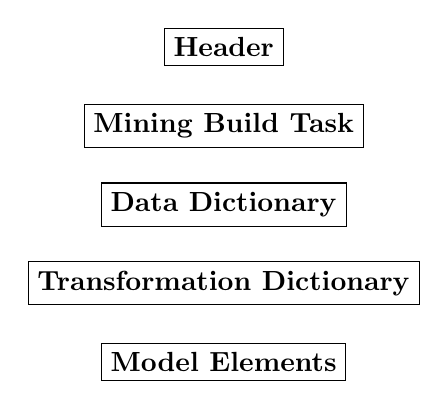
\begin{tikzpicture}
  \path (0,4) node [shape=rectangle,draw] {\textbf{Header}}
  (0,3) node [shape=rectangle,draw] {\textbf{Mining Build Task}}
  (0,2) node [shape=rectangle,draw] {\textbf{Data Dictionary}}
  (0,1) node [shape=rectangle,draw] {\textbf{Transformation Dictionary}}	
  (0,0) node [shape=rectangle,draw] {\textbf{Model Elements}};
\end{tikzpicture}
\caption{Structure of PMML model's XML document.}\label{fig:pmml_struct}
\end{figure}

The XML file describing PMML model has a structure depicted in Figure~\ref{fig:pmml_struct}. The structure of PMML file maps well to the typical machine learning inference problem as described in Chapter~\ref{chapter:ml_theory}. The \textbf{header} describes meta-data related to the model: when the model was created and what tool was used to create it. \textbf{Mining build task} is an optional element and is not required. It can contain any XML elements related to model creation or training. The information from this element is primarily used for visualization and maintenance purposes.  In \textbf{data dictionary}, fields used by the mining models and the types and ranges of those fields are defined. In PMML variables are called fields. \textbf{Transformation dictionary} defines data transformation function that can be used in any model that is part of PMML document. The function described in transformation dictionary might represent calculation for feature extraction required by machine learning model. One example of such operation is normalization of data where the data is transformed to have zero mean and unity variance during the training process and naturally same transformation must be applied when model is used to make prediction on new data. Next block in the structure of Figure~\ref{fig:pmml_struct} is a sequence of top level \textbf{model elements}. The PMML document can have 0 or more models, also called top-level models.  Model elements describe the model. Each model is required to have an attribute that is describe what kind of machine learning it performs: classification, regression, clustering, time series analyzing, sequences analyzing, association rules and mixed. The model also has an optional model name element. The consumer of the model can select what model to use based on its name. If no name is specified, the default behavior is to select first model from the sequence. The model has child elements that are common to all the models and some model specific elements. Fields used by the model are defined in mining schema. Output element contains output field elements that define what kind of values are returned from the model. Model statistics provides statistics related to the fields of the model. Targets holds information on target values. Local transformation define transformation, similar to transformation dictionary, that are local to the model. Model verification elements defines elements that can be used by the model consumer to results generated by the model are accurate regardless of the platform where the model is executed. Note that all elements except mining schema might not appear in PMML model description element. It is model dependent do they appear or not. The full list of supported models is provided in Table~\ref{tab:pmml_sup_models}. 

\begin{table}[h]
\begin{center}
\caption{Models that are supported by PMML format.~\cite{pmml_spec}}\label{tab:pmml_sup_models}
\begin{tabular}{c}
Association Rule Model \\
Bayesian Network \\
Baseline \\
Clustering \\
Gaussian Process \\
General Regression \\
k-Nearest Neighbors \\
Naive Bayes \\
Neural Network \\
Regression \\
Ruleset Model\\
Scorecard Model\\
Sequences \\
Text Models \\
Time Series \\
Trees \\
Vector Machine
\end{tabular}
\end{center}
\end{table}

Formally the structure and elements of PMML document are defined by XSD (XML Schema Definition) document. The schema doesn't define PMML document completely. There are also field naming conventions that have to be followed in order for PMML document to be valid, like requirement for fields in data dictionary and transformation dictionary to be unique. The reason for this requirement is that fields defined in these elements have global scope, they are visible to all models. If two fields are named the same then we have a name collision in the document, it will be impossible for application to known what field to use. A snippet from PMML definition is provide in Listing~\ref{list:pmml_snippet_spec}. The complete document description of the schema definition can be found at~\cite{pmml_xsd_schema}.
\newpage
\lstinputlisting[language=XML, basicstyle=\tiny, caption={Snippet from XML Schema specification.\label{list:pmml_snippet_spec}} ]{assets/pmml_schema_snippet.xml}

The PMML format was first introduced as part of data mining toolkit called Rattle (\texttt{R} Analytics Tool To Learn Easily). Later it was separated from Rattle into its own \texttt{R} package.~\cite{guazzelli2009pmml} Hence \texttt{R} has best support for PMML. It is also possible to export some of the machine learning models from \texttt{scikit-learn} to PMML using \texttt{sklearn2pmml} \texttt{Python} package. Some converters exits for other ML libraries but they are usually one man prototype projects on \texttt{GitHub} lacking proper documentation and capability description. Among notable ML libraries only Apache Spark has official support for PMML but just for 5 models types. Major deep learning libraries frameworks like TensorFlow, MXNet or PyTorch do not support PMML. Data mining groups that is in charge of developing and extending PMML has recently, in 2015, introduced new standard called Predictive Format for Analytics (PFA) that will most probably replace PMML~\cite{pfa}.  

\lstinputlisting[language=XML, basicstyle=\tiny, caption={PMML document representing linear model for predicting closing prise of Ethereum cryptocurrency based on the price of Bitcoin cryptocurrency.~\label{list:pmml_xml}} ]{assets/etherium_price_redict_model.xml}

To end this subsection on PMML we present an example of the linear regression model with input data standardization written in \texttt{scikit-learn} and converted to PMML using \texttt{sklearn2pmml} package. The python code and PMML document are provided in Listings~\ref{list:python_pmml_exmp} and~\ref{list:pmml_xml}. In order to port the model from \texttt{scikit-learn} we must use \texttt{PMMLPipeline} class that is inherited class from \texttt{scikit-learn}'s \texttt{PipeLine} class defined in \texttt{sklearn2pmml} package. The PMML pipeline is converted to PMML XML document using \texttt{skleran2pmml} function. 

\lstinputlisting[language=Python,style=protobuf, caption={Python code to convert linear regression model to PMML file from~\ref{list:pmml_xml}.~\label{list:python_pmml_exmp}} ]{assets/linear_model_pmml.py}

\subsection{Intelligence Layer}
Intelligence layer is a concept proposed in a paper~\cite{edgar2019} that came out off Ericsson research team in Finland. One central idea of intelligence layer is to decouple as much as possible the intelligence form application. One another important aspects are composition of intelligence services and life cycle management related to intelligence like intelligence setup and intelligence decomposition. But for our work the decoupling aspects are more relevant.

Currently intelligence is part of the application layer tightly integrated into application as part of its code. To update the intelligence usually the whole application must be updated. Another approach is to use intelligence as a cloud service. Whenever application needs some intelligent function like image classification or text translation it makes an HTTP request with the data to HTTP endpoint and gets back the result in the form of HTTP reply. This way intelligence is external to the application but other difficulties arise. Intelligence is not owned by application, sending data to cloud for evaluation and getting the result back might introduce latency and high bandwidth use, costs related to using cloud service and network bandwidth and privacy issues related to sending data to cloud. These difficulties can be avoided by having intelligence locally available, only connecting to cloud or internet for updates or to get new intelligence. And that is exactly one of the things that intelligence layer tries to provide as part of ecosystems. IL touches many more other aspects of machine learning platform, interested reader can review all the concepts in~\cite{edgar2019}.               


\clearpage

\section{Implementation}\label{chapter:implementation}\label{chapter:implementation}
In this chapter the proof of concept implementation of the intelligence layer is presented. The intelligence layer is implemented as D-Bus service running on Ubuntu Linux operating system. D-Bus is Inter-Process Communication (IPC) system that is used mostly on Linux based operating systems. The intelligence layer service reads ONNX models from the disk and creates D-Bus object for each model. User applications can access these object via interfaces defined by the IL service and call methods to execute the model and get back the results of inference. The concepts of D-Bus, like: service, object, interface, and how the protocol is used to create an intelligence layer service is explained in the next subsection. 

To execute ONNX models representing neural networks the nGraph~\cite{cyphers2018intel}  software library will be used. nGraph is used for converting neural networks represented with library specific format or library independent formats into nGraph's format and performing inference or training on the supported hardware backends. The hardware backend is a processing unit like GPU, CPU or some other computational hardware designed specifically for machine learning. We will be using only inference capabilities of nGraph. In principle some of the nodes from \texttt{ai.onnx.ml} operator set is also possible to implement using nGraph’s native set of operators, but we will leave it for future work.

\subsection{Base Architecture}
Diagram in Figure~\ref{fig:il_architecture} represents the high level architecture of intelligence layer service when it starts. During the initialization process IL reads ONNX model files from the special directory, each model is represented by single file with .onnx file extension. The directory is given to the program as a command line parameter. The process depicted in the diagram happens for every model found in the directory.

\usetikzlibrary{shapes.misc} 
\begin{figure}[h!]
\centering
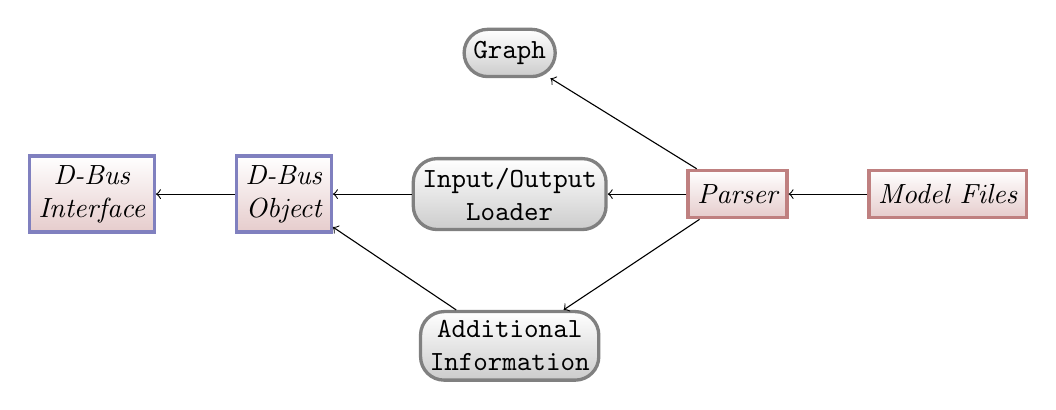
\begin{tikzpicture}[node distance=10mm,
nonterminal/.style={
% The shape:
rectangle,
% The size:
minimum size=6mm,
% The border:
very thick,
draw=red!50!black!50, % 50% red and 50% black,
% and that mixed with 50% white
% The filling:
top color=white, % a shading that is white at the top...
bottom color=red!50!black!20, % and something else at the bottom
% Font
font=\itshape
}, terminal/.style={
% The shape:
rectangle,minimum size=6mm,rounded corners=3mm,
% The rest
very thick,draw=black!50,
top color=white,bottom color=black!20,
font=\ttfamily},
dbus/.style={
% The shape:
rectangle,
% The size:
minimum size=6mm,
% The border:
very thick,
draw=blue!50!black!50, % 50% red and 50% black,
% and that mixed with 50% white
% The filling:
top color=white, % a shading that is white at the top...
bottom color=red!50!black!20, % and something else at the bottom
% Font
font=\itshape
}]

\node (m) [nonterminal] {Model Files};
\node (p) [nonterminal, left=of m] {Parser};
\node (l) [terminal, left=of p, align=center] {Input/Output \\ Loader};
\node (g) [terminal, above=of l] {Graph};
\node (a) [terminal, below=of l,  align=center] {Additional \\ Information};
\node (do) [dbus, left=of l, align=center] {D-Bus \\ Object};
\node (di) [dbus, left=of do,align=center] {D-Bus \\ Interface};

\path (m) edge[->] (p);
\path (p) edge[->] (l);
\path (p) edge[->] (g);
\path (p) edge[->] (a);
\path (l) edge[->] (do);
\path (a) edge[->] (do);
\path (do) edge[->] (di);
%\node (0,0) node [nonterminal] {Model Files} [draw]
%(-4,0) node [nonterminal] (-4,0) {Parser} 
%;


%  \path (0,0) node [nonterminal] {\textbf{Model files}}
%  (-1,0) node [shape=rectangle,draw] {\textbf{Graph}}
%  ;
\end{tikzpicture}

\caption{Architecture of IL service daemon.}\label{fig:il_architecture}
\end{figure}

ONNX model file is deserialized and parsed. Three pieces of information are crucial for creating an intelligent service out of deserialized ONNX model. The \textbf{graph} that describes the actual computations that must be performed on input data to produce a prediction or classification. The \textbf{input and output loaders} for converting data supplied by the user into presentation that can be fed to graph and converters the do a reverse operation. That is, converting the result produced by executing the graph on converted input data, to the format that can be sent back to the user. Last piece of information is \textbf{additional information} like documentation provided with the model, version and other information that is not directly related to computation. These three piece of information are represented in Diagram~\ref{fig:il_architecture} by rounded rectangles with corresponding titles with arrows ending at the boxes and diverging from parser rectangle. 

As depicted in the diagram additional information and input/output information is used to create a D-Bus object. Using terminology from Chapter~\ref{chapter:ml_theory} on intelligent agent, D-Bus object represents actuators and sensors of an intelligent agent. The intelligent agent can be identified with intelligent service that intelligent layer is providing for users to utilize. In theory we could consider other intelligent service as a user of other intelligent service to achieve for example reinforcement learning. But this topic is outside the scope of this thesis.           

\subsubsection{D-Bus IPC system}
D-Bus is a system for local IPC~\cite{dbus_spec}. It is built on top of \texttt{AF\_UNIX} sockets introducing interprocess communication concepts on the higher level of abstraction  like buses, services, clients, objects, interfaces, methods, signals and properties:  
    
\begin{itemize}
\item
A message \textbf{bus} is a source of services, or an application that allows other applications to communicate with each other. D-Bus system usually provides two buses: system bus and user bus. System bus is for system services and there is only one system bus on host Linux operating system. User bus is for user services and each user has his own bus. The IL service will communicate via user bus with its clients.  
\item
A \textbf{service} is a program that provides APIs to utilize the service on a bus. A service has a unique name specified in reverse domain notation. APIs for IL service are available at \texttt{fi.ericsson.nomadiclab.IntelligenceLayer}.   
\item
A \textbf{client} is a user application that uses APIs provided by a service. The client of IL service can view what intelligence services are available, query additional information about selected service and provide service with input to get back the result.  
\item
An \textbf{object} is identified by an object path and it belongs to a service. Service can have multiple objects that form directory tree like hierarchy. Object path looks like a file system path. For example an object path that is responsible for IL service managment might have a path \texttt{/fi/ericsson/nomadiclab/intelligence\_layer}. And for each intelligence service an object is created forming a list of object
\lstinputlisting[]{assets/il_service_tree.tree}
\item
Each object has one or more \textbf{interfaces}. Interface is defined by its members and provides APIs to utilize the object. A member can be a method, a signal or a property. Interfaces are identified by reverse domain name notation. Interface for image classification  model from previous example might be \texttt{fi.ericsson.nomadiclab.IntelligenceLayer.Classifier}     
\item
A \textbf{method} of an interface is a function that can take inputs and produce an output. For example \texttt{Classifier} interface might have \texttt{DoPrediction} method method to classify input data. A set of parameters that a method takes and returns is specified by method's \textbf{signature}. The signature is encode as a series off characters. For \texttt{DoPrediction} method of \texttt{Classifier} interface, signature might be \texttt{s} for input and \texttt{as} for output, telling the user of the method that \texttt{DoPrediction} takes string as input and returns array of strings to the client that invoked the method. Input string can represent a link to a resource, for example a file system path to an image. Output might be an array of all categories sorted in descending order starting with category with the highest classification score.             
\item
Methods are for one-to-one, request-response communication between a client and a service. A \textbf{signal} can be used for one-to-many, or also one-to-one, notifications. For example IL service might send a signal to all the clients that a new model is introduced or that one of existing models was updated to a newer version. We can also imagine having intelligence service that do not require and input from the client and just send the client result of some computation based on data that it receives from the system. 
\item 
A \textbf{property} is just a variable. The type of property is defined with a signature using the same syntax as for methods. Interface for intelligence service object might have properties exposing meta information provided by ONNX model like documentation string of a model and a model version.        
\end{itemize}

The users of IL service, that are clients, can introspect which objects are available under the models path and use interfaces provided by those objects to call methods that execute the machine learning model and get back the result or examine properties that contain description of the model and some additional information about the model.       


\subsubsection{The Graph}
The nGraph software library is used to extract the graph from ONNX model. nGraph allows us to convert graph that is part of ONNX model to the graph represented by nGraph's  IR format, compile the converted graph and execute produced code on the hardware that nGraph supports. 

nGraph can be used for training and inference~\cite{cyphers2018intel}. Training means calculation of gradient with respect to neural network parameters. Four our implementation of intelligence layer we are only interested in inference. 

In order to run inference code we must ask nGraph to allocate memory for input and output, fill memory reserved for input with data, then after the graph is applied to data, we have to read the result and send it to client. The D-Bus method call used by client for invoking inference execution might have a signature specifying that client must supply raw data as a parameter to the method call. The raw data is suitable if model provides a purely computational service. Array of numbers goes in and modified arrays of numbers is returned to client. Since intelligence layer is assumed to be smarter other input data type might be a string, representing a link to a resource. Resource might be a file system path, url or path to the device. The IL must have capability to extract raw data from the resource and write to memory allocated by nGraph for input. Our current implementation only support strings pointing to resources on a file system. For example a path to a location for image that client wants to classify.      

\subsubsection{Input and Output Loaders} 
In nGraph computational graphs are represented by functions. Function takes as input a multidimensional array filled with numbers. The data represented by an array of numbers does not have any semantic meaning. To give semantic meaning to data ONNX has an experimental feature called denotations. A tensor in ONNX can have optional denotation represented by string literal. Intelligence layer uses this denotations to use correct loaders to extract raw data, pointed to by resources that are supplied by a calling client with a method call, and fill input memory of the nGraph's function. After nGraph function is executed we need to use produced data, that is again purely numerical, for preparing a sensible reply to user. For that again input tensor denotation is used.        
  
Denotations are also used to assign a correct interface to D-Bus object created for a model. For example if input tensor is denotated as image and output tensor is denotated categorical then we know that model object requires classification interface. If denotation for tensor is missing we create interface for regression.               
                  
\subsubsection{Other information}
Client might be interested in a short description of a model or what kind of input model expects. These information can be conveniently presented as properties of D-Bus model object. In the implementation of IL in this work we provide almost all descriptive model information available in \texttt{ModelProto}:
\begin{itemize}
\item
Version of the ONNX IR
\item
Tool used to produce model
\item
Version of the tool use to produce model
\item
Domain to which model belongs
\item
Name of the author if available
\item
Input Denotation
\item
Output Denotation
\end{itemize}

\subsection{Software design}
In order to deliver continuous operation and low latency the intelligent layer service must be implemented as a concurrent program. It is assumed that IoT device supports multithreading. In concurrent system different procedures are running on multiple threads of execution. The procedures need to communicate with each other and share different resources. An additional complication comes from using \texttt{C++} as implementation language that was chosen for implementing IL. \texttt{C++} allows to write efficient code with low overhead but it is regarded as complex language, requiring a lot of low level knowledge to create concurrent programs. 

One way to implement concurrent program is to use raw threads and synchronization mechanism like mutexes and conditional variables. Other approach that I chose for my implementation is to use actor model~\cite{agha1985actors}. In actor model many system components can be represented as actors. Actors might be \texttt{C++} objects that run on the same or different threads. Actors communicate with each other by exchanging messages. Based on received messages actor react by sending new message or doing some computations. Actors don't share any state among each other hence making race condition that are common source of bugs in concurrent programs less probable. All mechanism required to synchronize the message exchange is handled by framework providing the implementation of the actor model.          
I my implementation I use \texttt{SObjectizer} \texttt{C++} actor model framework. It provides enough features to implement intelligence layer. One restriction that \texttt{SObjectizer} has compared to some other actor frameworks is that it doesn't allow distributing actor among different computers scattered over computer network. But for my implementation this functionality is not required.      
     
The more detailed diagram, based on the actor model, of architectural diagram presented in Figure~\ref{fig:il_architecture} is presented in Figure~\ref{fig:il_architecture_2}.   
\begin{figure}[h!]
\centering

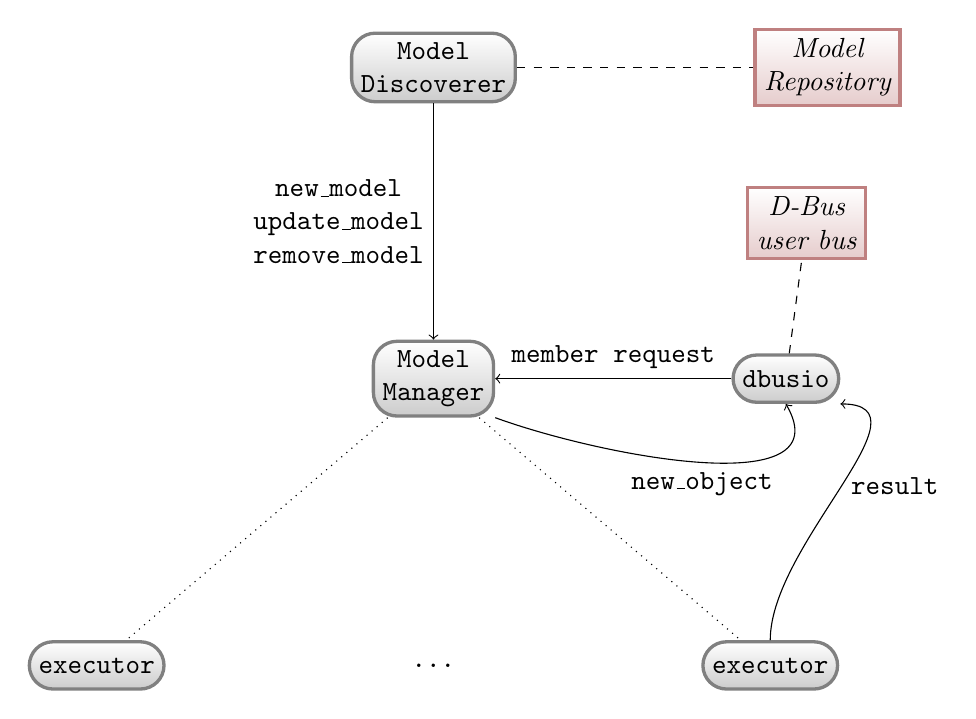
\begin{tikzpicture}[node distance=30mm,
resource/.style={
% The shape:
rectangle,
% The size:
minimum size=6mm,
% The border:
very thick,
draw=red!50!black!50, % 50% red and 50% black,
% and that mixed with 50% white
% The filling:
top color=white, % a shading that is white at the top...
bottom color=red!50!black!20, % and something else at the bottom
% Font
font=\itshape
},
 actor/.style={
% The shape:
rectangle,minimum size=6mm,rounded corners=3mm,
% The rest
very thick,draw=black!50,
top color=white,bottom color=black!20,
font=\ttfamily},
dbus/.style={
% The shape:
rectangle,
% The size:
minimum size=6mm,
% The border:
very thick,
draw=blue!50!black!50, % 50% red and 50% black,
% and that mixed with 50% white
% The filling:
top color=white, % a shading that is white at the top...
bottom color=red!50!black!20, % and something else at the bottom
% Font
font=\itshape
}]

\node (md) [actor, align=center] {Model \\ Discoverer};
\node (mm) [actor, align=center, below=of md] {Model \\ Manager};
\node (dbusio) [actor, align=center, right=of mm] {dbusio};
\node (dots) [below=of mm ] {\texttt{...}};
\node (ex1) [actor, left=of dots ] {executor};
\node (exn) [actor, right=of dots ] {executor};
\node (fs) [resource, right=of md, align=center] {Model\\ Repository};
%\node (dbus) [resource, below=of fs, align=center] {D-Bus\\ user bus};
\node (dbus) [resource, align=center] at ($(fs)!0.5!(dbusio)$) {D-Bus\\ user bus};

\path (md) edge[->] node[left,align=center]
{\texttt{new\_model}\\\texttt{update\_model}\\\texttt{remove\_model}}
 (mm);
\path (mm) edge[<-] node[above,align=center] 
{\texttt{member request}}
 (dbusio);
\draw [<-] (dbusio.south) to [out=300,in=340] node[below] {\texttt{new\_object}} (mm.south east);

\draw [->] (exn) to [out=90,in=0] node[right] {\texttt{result}} (dbusio.south east);

\path (mm) edge[dotted] (ex1);
\path (mm) edge[dotted] (exn);
\path (md) edge[dashed] (fs);
\path (dbusio) edge[dashed] (dbus);  
\end{tikzpicture}

\caption{Actor model based design of intelligence layer. Arrows represent message sending. Dotted lines represent creation of executor actors by model manager. Dashed lines represent access to external resource like file system and D-Bus user bus. }\label{fig:il_architecture_2}
\end{figure}
The diagram in Figure~\ref{fig:il_architecture_2} presents four different types of actors: \texttt{model discoverer}, \texttt{model manager}, \texttt{dbusio} and \texttt{model executor}. Exactly one instance of actor exits for discoverer, manager and dbusio. Zero or more instances of executor actor are dynamically created by model manager when users make request to execute the model via dbusio actor. After executing the nGraph model function and returning the result to dbusio, model executors actors are destroyed.         

Model discoverer scans the model repository periodically to detect changes. Model might be added, removed or updated. When model discoverer detects change to the repository, it parses the ONNX model files if model was updated or added and sends appropriate message to model manager. As is presented in the Figure~\ref{fig:il_architecture_2} discoverer can send three different messages:
\begin{itemize}
\item \texttt{new\_model} to add new model to the model list of model manager.
\item \texttt{update\_model} to update existing model.
\item \texttt{remove\_model} to remove model from the list of model manger.  
\end{itemize}

\texttt{new\_model} and \texttt{update\_model} messages contain all information required to execute the model: like model name, the types of input and output, nGraph function and other information related to model like documentation string. For removing the model all these information is not required and only name of model is attached to the message. 

When the model manager receives a \texttt{new\_message} messages it adds model to its list of models and sends \texttt{dbusio} actor \texttt{new\_object} message to create a D-Bus object for the model. \texttt{dbuisio} exposes the appropriate interface of the object to clients of IL service. The member invocations requested by clients are routed to model manager. These invocation are represented by \texttt{member request} in Figure~\ref{fig:il_architecture_2} but they might be implemented by multiple different messages. 

For the D-Bus object's property requests or method calls that do not require any computation model manager actor doesn't create executor actor. If method request requires execution of nGraph function then model manger creates executor actor potentionaly on a different thread of execution so that model manger can still handle incomming messages while executor is doing computations. When executor is done, it sends \texttt{result} message to dbusio actor to relay this reply to client that invoked the method.                      
\newpage


\section{Results and Conclusions}\label{chaper:results}
It is clear that ONNX at the moment is an appropriate and popular format for representing neural network machine learning models intended for inference purposes. Many state-of-the-art deep learning frameworks support ONNX to some extent and new compilers and runtime capable of executing ONNX NN models on variety of compute hardware, ranging from general purpose hardware like CPUs and GPUs to special purpose like Intel's Nervana~\cite{cyphers2018intel} chip designed to accelerate NN computations, emerge all the time. The list, available at ONNX's Web-page~\cite{onnx_tools}, of frameworks, run-times, compilers that ONNX team claims to support ONNX format is getting updated frequently. One recent development is the release of ONNX Runtime as an open source project by Microsoft. ONNX Runtime is a software library for executing ONNX models. In the Microsoft's blog post~\cite{onnx_runtime} accompanying the release of the project it is claimed that ONNX Runtime has full support for ONNX version 1.2 and later, including \texttt{ai.onnx.ml} set of operators.  
ONNX Runtime is first runtime to support both sets of operators \texttt{ai.onnx} and \texttt{ai.onnx.ml}. ONNX Runtime would have been better solution compared to nGraph as an model executor for the implementation that was introduced in Chapter~\ref{chapter:implementation}. But the ONNX Runtime was released after the decision has been made to use nGraph for the implementation and for that reason it was decided to continue with nGraph.

If we compare the lists of available operators from \texttt{ai.onnx.ml} domain in Appendix to the list of models in Table~\ref{tab:common_model_iot} we can see lists have only four common models: linear regression, SVM, decision trees and bagging. Bagging can be considered and ensemble of trees. Most of the other operators of \texttt{ai.onnx.ml} domain are for data pre-processing and data post-processing. On the  other hand it must be kept in mind that, in theory, the operators from different domains can be mixed, if model executor supports them both. Using operators from the default domain \texttt{ai.onnx}, it is possible to express any computations that do not require back-loops. So it can be hypothesized with high probability that most of the operators from Table~\ref{tab:common_model_iot} are implementable in ONNX, for example if we are not considering training, PCA from section~\ref{sec:ml_in_iot} is just a matrix multiplication operation. Even if some operation is not implementable with standard set of operators, ONNX can be extended with custom domains of operators and then it will depend on the executor what operators it can and can't run. 

On the other hand if we look at Table~\ref{tab:pmml_sup_models} presenting models that are supported by PMML we can see that it is more compatible with Table~\ref{tab:common_model_iot}. One might think that for that reason PMML is better format for representing machine learning models. But it must be taken into account that PMML has been around since 1999, when version 1 of the format was released, and until these days PMML is not widely adopted especially from the tools used to create and execute neural networks. The protocol buffer format is superior to XML in terms of size of serialized models and parsing speed. For that reasons, we think that ONNX is a better choice for representing also classical machine learning models and not just neural networks. The author of these thesis do realize that more systematic comparison of PMML and ONNX must be conducted in order to decide with format is better but it would necessary take more space and resource that are not available and hence we leave it for feature work. Right now it looks clearly that industry tends to prefer ONNX over PMML with big corporation like Microsoft and Facebook driving development of ONNX.

\subsection{Preparing ONNX models as service}     
To test the implementation we needed an ONNX model. The place where one can find ready made pre-trained ONNX models is called ONNX Model Zoo~\cite{onnx_model_zoo}. It is a GitHub repository with the models that have been developed with some framework, like MXNet, and then exported to ONNX. For each provided model there is also a description available, describing what framework was used to create the model, where the data that was used for training come from and how pre-process and post-process the raw data for model execution.

We decide to use version 2 of the ResNet~\cite{he2016deep} image classification neural network model for our testing purposes. The model takes image data as input and outputs the class of the major object in an image. The model was trained on the ImageNet dataset which contains images from 1000 classes. We used largest available model Resnet-152 that is approximately 220 MB is size and is most accurate. Image classification is an important use case for IoT. One can image camera monitoring the production line for faulty products taking a snapshop image of a product and requesting a prediction from intelligence layer service to classify the product as good or bad.        

We couldn't use model as it was provided because it was assumed that pre-processing and post-processing procedures are done in code. Model was just expecting an $1 \times 3 \times 224 \times 224$ dimensional tensor as input and producing $1000$ dimensional tensor as output. Input tensor should contain data of color image and output tensor score for each class. It was assumed that user of ResNet ONNX model will know enough information about the model to load an image in some format, for example PNG, extract pixel values for each channel using some libraries and normalize pixel values to range $[0,1]$. Same assumption was made for the output. It was users job to download the file with all the names of categories and connect result with categories. 

In order to fix these issues we had to add computational pre- and post-processing nodes. For preprocessing we did standardization of the data and for post-processing we converted score to probabilities with softmax function.

In order for intelligence layer to know that model expects an image prepared in a particular way we had to denotate input tensor and all the dimension of an input tensor. Denotating dimensions was less import to us, but we did it for completeness. Denotating in our context means giving semantic description to tensors, so that intelligence layer service can understand the meaning of a tensor and use appropriate loader. The ONNX has an experimental proposal for detonating tensors that is not part of the official release yet~\cite{onnx_denotations}. For that purpose \texttt{TypeProto} message has \texttt{denotation} field that is a string. Three types of denotation are available: \texttt{TENSOR}, \texttt{IMAGE}, \texttt{AUDIO}, \texttt{TEXT}. Out of these four, only \texttt{TENSOR} and \texttt{IMAGE} have a somewhat complete definitions. Tensor doesn't require any denotation. Same goes for dimension denotations. \texttt{Tensor} protocol buffer message has \texttt{TensorShapeProto} field that is a array of \texttt{Dimension} messages that have \texttt{denotation} field. The definition for dimension denotations are not well formalized yet. 


The denotation for type and dimensions of input tensor of the modified ResNet model are provide in Figure~\ref{fig:input_denotation}. As we can see model expects and \texttt{IMAGE} as an input. The format of the image is specified on right side of Figure~\ref{fig:input_denotation}. Using this information intelligence layer will know that it should image has a specific pixel format, color space and that it should normalize pixel values to range $[0, 1]$ by scaling data from each color channel by $255$. Dimension also have meaning but current version for intelligence layer disregards them.    

\begin{figure}[h!]
\centering
\begin{tikzpicture}
\node at (-4,0) {\lstinputlisting{assets/input_denotated.model}};
\node at (4,0)  {\lstinputlisting{assets/input_denotated_meta.model}};
\end{tikzpicture}

\caption{Textual representation of input denotation for ResNet model's input. Left side is snippet that represents input of the graph. On the right side the key-value pairs of the \texttt{meta\_data} field are presented related to \texttt{IMAGE} type.}\label{fig:input_denotation}
\end{figure}

For output tensor, of our modified ResNet model,that is probability for categories we had to invent our own semantic type. We named it \texttt{CATEGORICAL\_PROBABILITY}. To denotate some tensor as \texttt{CATEGORICAL\_PROBABILITY} we must set its denotation filed to \texttt{CATEGORICAL\_PROBABILITY} and add all the categories as map from category identifiers to category names in \texttt{meta\_data}. Textual representation of output tensor is presented in Figure~\ref{fig:output_denotation}        

\begin{figure}[h!]
\centering
\begin{tikzpicture}
\node at (-4,-2) {\lstinputlisting{assets/output_denotated.model}};
\node at (3,2)  {\lstinputlisting{assets/output_denotated_meta.model}};
\end{tikzpicture}

\caption{Textual representation of output denotation for ResNet model's output. Left side is snippet that represents input of the graph. On the right side the key-value pairs of the \texttt{meta\_data} field are presented related to \texttt{CATEGORICAL\_PROBABILITY} type.}\label{fig:output_denotation}
\end{figure}

The model was prepared for consumption by intelligence layer using Jupyter Notebook. In the notebook ONNX model was imported into MXNet and missing operators were added for pre- and post-precessing. After this, model was exported again to ONNX and then loaded again to denotate the input and output tensors. For that \texttt{onnx} \texttt{Python} package was used that is part of official ONNX release.   

\subsection{Testing Implementation} 
After creating an implementation and modifying the model so that it can be served by intelligence layer we tested with the standard command lines tools provided by Ubuntu Linux distribution to interface with D-Bus objects and wrote a short \texttt{Python} program that also uses the service. 

The work that we did proofs that it is possible to use ONNX as the format for delivering complete machine learning solutions. Our approach is different from other model serving solution which are usually HTTP end-points and are not part of the operating systems. Preparing such an HTTP endpoint usually requires to write computer program that transforms input and output data. In our approach model are complete and all the complexity for IO transformation and API serving is hidden behind intelligence layer as long as creator of a model denotates the input and output tensors correctly.        
 
\subsection{Feature Work}   
\textbf{TD}\\   
\textbf{Below are just notes for myself.}     \\            
Do a more complete comparison between PMML and ONNX.      
Implment more ideas from Intelligence Layer related to lifecycle managment of machine learning models.
Port more ONNX models as intelligence layer services 
%\section{Results and Analysis}
\\
%\section{Conclusions}
Future work
Do a systematic research of how well ONNX is supported. 
Extend to support ai.onnx.ml 
To service discovery for example notification for clients when new models are appear in the special directory.
Life cycle management.    
https://azure.microsoft.com/en-us/blog/onnx-runtime-is-now-open-source/
While writing these thesis a ONNX runtime emerged that would have been perfect replacement of nGraph because it also support ONNX-ML profile. This shows how rapid is the development of these are of machine learning is.

Increasing performance of IL by distribution taks further on discoverer and executors.
D-Bus supports only double-precision types. Extending it with single-precision is important.      
%\section{Yhteenveto}




\clearpage
%% Lähdeluettelo

\thesisbibliography
\bibliography{references}{}
\bibliographystyle{ieeetr}



\clearpage
\thesisappendix
\section{Lists of ONNX Operators\label{appendix:operatorlist}}
In this appendix the list of ONNX operators from both standard operator sets are provided. First listing has the operators from \texttt{ai.onnx} set. Second listing  presents operators from \texttt{ai.onnx.ml} set.  
\lstinputlisting[language=protobuf3,style=protobuf]{assets/aionnx.txt}
\lstinputlisting[language=protobuf3,style=protobuf]{assets/aionnxml.txt}
\end{document}